\chapter{La perception sensible}
%chapitre V
%70. La connaissance sensible, — 71.Sensation et perception. — 72, Conditions
%de la sensation. — 73. Lois de la sensation ; la Psychophysique. —
%74. Les trois sensibilités. — 75. La sensibilité intéroceptive. — 76. La sensibilité
%proprioceptive. — 77. La sensibilité extéroceptive : A. sens impressionnables
%par contact direct ; B. sens impressionnables à distance. — 78.
%Valeur des différents sens. — 79. Rôle de la sensation. — 80. La notion de
%« sensation ». — 81. La perception des « formes ». — 82. Discussion du Gestaltisme.
%— 83. Du syncrétisme aux objets. — 84. La construction des
%objets. — 85. Les cadres sociaux de la perception. — 86. La perception individualisée.
%— 87. « L'éducation des sens ». — 88. Les erreurs de la perception.

\section{La connaissance sensible}% 70.
Nous connaissons le monde
extérieur \textbf{\textit {par nos sens.}} C’est pourquoi certains philosophes ont prétendu
ramener toute la connaissance aux messages que ces sens nous
apportent. « Il n’est rien dans l’entendement, disait un adage scolastique,
qui n’ait été auparavant dans la sensibilité : {\it nihil est in intellectu
quod non prius fuerit in sensu} » et, au {\footnotesize XVIII}$^\text{e}$ siècle, Condillac ira
jusqu’à faire de la sensation l’élément unique dont les combinaisons
engendreraient toute notre vie mentale : ce sera le {\it sensualisme} ou
doctrine de la « {\it sensation transformée} » qui est d’ailleurs une des formes
de l’{\it atomisme psychologique} (\S 37, fin). Plus prudemment, Aristte
avait dit que « celui qui n’aurait pas la sensation ne pourrait
rien connaître », mais que cependant « la sensation n’est pas le savoir ».
— Imaginons-nous en effet {\it réduits à nos sens seuls}. Nous entendrions
des bruits et des sons; nous apercevrions des formes ombrées et
colorées tantôt fixes, tantôt mouvantes; nous respirerions des
odeurs, etc. Mais tous ces messages n’auraient pour nous {\it aucun sens}.
%81
Cet état n’est pas absolument imaginaire ; c’est sans doute, approximativement,
celui du tout jeune enfant, du nouveau-né : il entend,
voit, sent à peu près comme nous (sauf, pour la vision notamment,
certains phénomènes d’adaptation et d’accommodation) ; mais il ne
\textbf{\textit {comprend}} pas les messages de ses sens. Ceux-ci ont donc besoin
d’être {\it interprétés par l'esprit} pour acquérir une \textbf{\textit {signification.}}

\section{Sensation et perception}% 71.
Ceci nous conduit à la distinction
classique de la sensation et de la perception. La \textbf{\textit {sensation}}
serait l’{\it état de conscience élémentaire consécutif à une impression faite
sur l’un de nos organes sensoriels}. La \textbf{\textit {perception}} serait la sensation
{\it interprétée}, devenue {\it significative}, c’est-à-dire impliquant la notion
d’{\it un certain objet}, extérieur à nous, localisé dans l’espace, etc. Prenons
un exemple. Je travaille tranquillement à mon bureau lorsque tout
à coup j'entends un bruit assez aigu, une sorte de crissement : simple
{\it sensation}. Mais tout aussitôt et sans avoir besoin de réfléchir, je
pense que c’est le coup de frein brusque d’une auto dans la rue et
je me précipite à la fenêtre pour voir s’il n’y a pas eu d’accident :
{\it perception}. Mais le nouveau-né, lui, aurait simplement entendu le
bruit.

On verra par la suite que cette distinction classique de la {\it sensation}
et de la {\it perception} est quelque peu battue en brèche par certaines
doctrines contemporaines : théorie de la {\it Gestalt} et phénoménologie
La sensation serait, en effet, la pure {\it intuition sensible} telle que nous
l'avons définie au \S 60. Mais nous avons déjà montré alors quelles
réserves appelle cette notion, bien que ces réserves aillent, dans une
certaine mesure, en sens inverse des thèses soutenues par la Phénoménologie
(voir \S 80). Les exemples que nous venons de donner
suffisent à montrer cependant que la distinction entre sensation et
perception n’est pas dénuée de toute valeur et, pour la commodité
de l'analyse, nous commencerons par étudier les problèmes relatifs
à la sensation pure.

\section{Conditions de la sensation}% 72.
La sensation, fait psychique,
a des conditions {\it physiques} et des conditions {\it physiologiques}. Lorsque,
par exemple, j'entends un bruit ou un son, il y a là d’abord un phénomène
{\it physique}, dont l'étude relève de l’Acoustique : le bruit ou le
son en tant que vibration de l’air. Nous appellerons \textbf{\textit {excitant}} ou
\textbf{\textit {stimulus}} la cause {\it }physique de la sensation
{\scriptsize (Pour certains sens, comme ceux du goût ou de l’odorat, l’excitant est d'ordre
chimique. Dans la sensibilité intéroceptive (\S 75), l’excitant, étant interne, est d'ordre
physiologique)}.
%82

Cet excitant produit dans l’organe sensoriel, ici l'organe de l’ouie,
un ensemble de phénomènes, d’ordre {\it physiologique} cette fois et dont l’étude
relève des Sciences naturelles : nous désignerons tout cet ensemble par le terme
d'\textbf{\textit {impression.}} Un organe sensoriel est essentiellement constitué par des
{\it terminaisons nerveuses sensitives}, libres ou bien encapsulées dans des
corpuscules (tels les corpuscules du tact) ou même pourvues de cellules
sensorielles spéciales (telles les cellules auditives de l’organe de Corti ou
les cellules à cônes et à bâtonnets de la rétine) : ce sont ces terminaisons
qui reçoivent l'{\it impression} proprement dite faite par l'excitant. Cette
impression est conduite au cerveau par le nerf sensitif. Comme on l’a vu
(\S 29 B), chaque sens a, dans le cerveau, sa {\it zone réceptrice}
spéciale. C’est ainsi que les impressions auditives se projettent
dans la région temporale ; les impressions visuelles, dans la
région occipitale, chaque hémisphère étant relié à la moitié du
côté correspondant des deux rétines et les quadrants supérieurs se projetant
au-dessus,

les quadrants inférieurs au-dessous de la scissure calcarine
(face interne du lobe occipital), etc. —
Il y a lieu de remarquer qu’on peut déjà observer, du point de vue
anatomique même, une certaine hiérarchie entre les différents sens,
ainsi que le montre la figure 9 : dans les sens supérieurs, comme la
vue (E), pourvus de cellules différenciées, on voit les neurones sensitifs,
non seulement périphériques, mais même centraux, venir se situer
vers la périphérie, à tel point qu’on a pu dire que le nerf optique est
une « véritable partie des centres nerveux » (Chauchard).

\begin{minipage}[c]{.45\linewidth}
\begin{center}
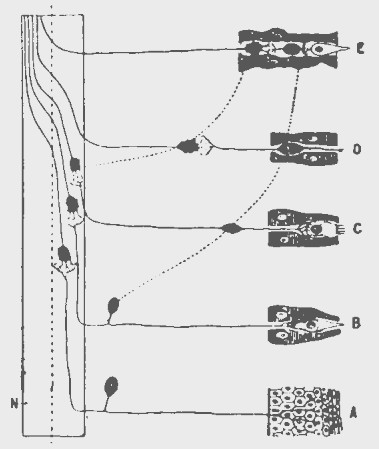
\includegraphics[scale=0.3]{./05_sensible/009}
\end{center}
Fig. 9. — Schéma des organes des sens
(D'après Gley, Traité de Physiologie, J.-B. Baillière, éd.).
\end{minipage}
\hfill
\begin{minipage}[c]{.45\linewidth}
N, centres nerveux ; A, tact; B, goût;
C, ouïe; D, odorat ; E, vue. — Les cellules 
sensorielles (absentes pour le tact et l'odorat) 
sont figurées en clair ; les neurones sensitifs
périphériques, en noir avec un noyau ; 
les neurones sensitifs centraux, en noir 
sans noyau. La ligne pointillée de droite
marque le déplacement vers la périphérie des neurones périphériques à partir de celui 
de l'audition (C) ; la ligne supérieure, le
même déplacement pour les neurones centraux à partir de celui de l'odorat (D).
\end{minipage}


%83
\section{Lois de la sensation; la Psychophysique}% 73.
Les lois de
la sensation seront donc de trois sortes, selon qu’il s’agit de ses rapports :
{\it A.} avec l’excitant; {\it B.} avec l'impression physiologique ;
{\it C.} avec les autres faits de conscience antécédents ou concomitants.

{\it A.} Lois {\it psycho-physiques}. Les premières sont les lois dites « psycho-physiques ».
1° La \textbf{\textit {loi du seuil,}} qu’on retrouvera à propos du comportement
(t. II, ch. I), s’applique à la sensation : il existe pour chaque
sens une intensité {\it minima} de l’excitant, appelée {\it intensité liminaire}
(latin : {\it limen}, seuil), au-dessous de laquelle il n’y a pas de sensation.

\vspace{0.24cm}
{\footnotesize 
La Psychologie de laboratoire s’est appliquée à déterminer ces \textsf{\textit {seuils
sensoriels,}} et l’on a pu obtenir pour chaque sens une valeur moyenne du
seuil. Mais ces valeurs n’ont rien d’absolu. Il y a naturellement des
différences individuelles. La sensibilité tactile est très inégalement répartie
selon les différentes régions du corps : très grande au bout des doigts
(2 mg à la face interne, 15 mg au dos de l'index) et à la pointe de la
langue, elle est très faible pour la peau du dos. La sensibilité visuelle n’est
pas la même pour les différentes radiations : dans des conditions moyennes
d’éclairement, elle est maxima pour une longueur d'onde de 55 µ (vers le
jaune-vert). Le goût est plus sensible à l'amer qu’au sucré. La sensibilité
olfactive varie beaucoup selon les odeurs, etc. D'autre part, par suite d'un
phénomène d'adaptation, le seuil est plus bas quand on expérimente par
{\it diminution} progressive de l’excitant que lorsqu'on le fait croître. Enfin il
faut tenir compte de la durée de l’excitation : il existe une certaine durée,
dite {\it temps utile}, au delà de laquelle seule le seuil devient invariable.}
\vspace{0.31cm}

2° La seconde loi est celle du \textbf{\textit {seuil différentiel}} : de même qu’un
excitant trop faible n’est pas senti, une {\it variation} d’intensité de l’excitant
doit atteindre un certain seuil pour qu’on sente la différence.
Les recherches poursuivies vers 1830 par le physiologiste allemand
E.-H. Weber (1795-1878) ont établi qu’{\it il existe, pour chaque espèce
de sensation, un rapport constant entre l'intensité de l’excitant initial
et la variation minima qu’il faut lui faire subir pour que la différence
soit sentie} : c’est ce qu’on appelle la \textbf{\textit {loi de Weber}} (bien qu'elle ait
été énoncée dès 1760 par le physicien français Bouguer pour les
sensations lumineuses). Autrement dit, la « constante de Weber »
qui mesure le seuil différentiel, n’est pas une valeur absolue : c’est un
rapport. Elle est, par exemple, de 1/20 pour les sensations tactiles, ce
qui veut dire que, si j’ai sur la main un poids de 20 g, celui-ci devra
être augmenté d’au moins 1 g pour que je sente la différence; mais,
si je pars d’un poids de 40 g, il devra être augmenté d’au moins
2 g. Cette loi vaut surtout pour les intensités moyennes.

Se fondant sur ces résultats, le philosophe G.-Th. Fechner (1801-1887)
crut pouvoir tirer de là une méthode de \textbf{\textit {mesure}} de la sensation,
point de départ de toute une science qu’il nomma la \textbf{\textit {Psychophysique}}
%84
(1860). Il admit ce postulat que les modifications tout juste sensibles
que subissent rios sensations quand on augmente l’excitant et qui
correspondent au seuil différentiel, sont toutes égales à la sensation
qui correspond à l'intensité liminaire, prise pour unité. Il énonça
alors la loi de Weber sous cette forme : pour que la sensation subisse
ainsi des accroissements uniformes, c’est-à-dire pour qu’elle varie
en {\it progression arithmétique} (comme les nombres 0, 1, 2, 3, etc.), il
faut faire varier l’excitant en {\it progression géométrique} (comme les
nombres 4, 10, 100, 1 000, etc.), ce qui peut encore se formuler : {\it la
sensation varie comme le logarithme de l’excitant. Ce fut la} \textbf{\textit {loi
logarithmique}} {\it ou} \textbf{\textit {loi de Fechner.}}

\begin{minipage}[c]{.45\linewidth}
Rapports de la sensation S (en ordonnées)  et de l'excitant E (en abscisses) selon 
une échelle logarithmique. Si la loi de Fechner était exacte, les accroissements 
de la sensation s'effectueraient selon la droite en pointillé Elle s'effectue en 
réalité selon une courbe en S. Mais pratiquement cette courbe coïncide avec  
la droite pour les valeurs moyennes. 
\end{minipage}
\hfill
\begin{minipage}[c]{.45\linewidth}
\begin{center}
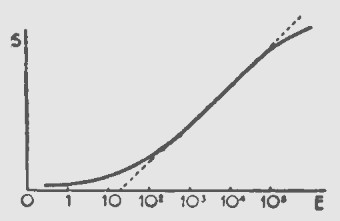
\includegraphics[scale=0.6]{./05_sensible/010}
Fig. 10. — La loi de Fechner.
(D'après Piéron, Psychologie expérimentale, (Coll. Armand Colin.)
\end{center}
\end{minipage}

\vspace{0.24cm}
{\footnotesize 
Ces conclusions de Fechner ont
été très discutées. Bergson y a
opposé une objection de principe :
les sensations, comme tous nos états
de conscience, seraient purement
{\it qualitatives}, et ce serait par une illusion matérialisante que nous
transporterions le caractère quantitatif de la cause physique ou physiologique
(intensité de l’éclairement, de l'effort musculaire, etc.) dans le domaine
de la sensation elle-même. Mais cette opposition absolue qu'établit Bergson
entre {\it quantité} et {\it qualité} est peu fondée : tout ce que la science a
appris à traduire par une quantité, et le nombre lui-même (voir le
\S 249 A), est apparu d’abord à la conscience naïve comme purement qualitatif.
— D’autres objections ont porté sur le caractère arbitraire du postulat
de Fechner. Mais toute mesure implique certaines conventions : n’est-ce
pas une convention de mesurer la vitesse d’un corps qui tombe, par l’espace
parcouru en une seconde, et cette vitesse est-elle davantage une somme de
vitesses plus petites qu'une sensation un total d'unités de sensation ?}
\vspace{0.31cm}

 



L'erreur de Fechner était ailleurs : elle était, au fond, dans la
notion même d’une « psychophysique », c’est-à-dire d’une {\it relation
directe entre l’excitant physique et la sensation comme processus conscient}.
Physicien avant d’avoir été philosophe, Fechner a méconnu en
effet qu’entre l’un et l’autre, s’intercale un intermédiaire, qui est
notre corps avec toute la complexité de ses organes, de ses voies
nerveuses, de son cerveau. La loi de Fechner exprime donc, en réalité,
un rapport entre l’excitant physique et la {\it réaction de notre sensibilité
%85
organique}, que la sensation consciente ne traduit qu’en gros et peu
fidèlement ; et en effet son graphique correct (fig. 10) donne une courbe
analogue à celle de toutesles réactions organiques (t. II, fig. 2 ). Avec ces
réserves, elle fournit une approximation suffisante pour la pratique,
et la meilleure preuve de sa valeur est qu’elle a été appliquée empiriquement
avant d’être connue scientifiquement
{\scriptsize (On sait que les premiers astronomes avaient classé les étoiles, selon leur éclat
apparent ou magnitude, en étoiles de 1r°, 2e, 3, etc., grandeur ; or cette hiérarchie
correspond en réalité à une progression géométrique décroissante : chaque classe est
2,5 fois plus brillante que celle qui la suit. — De même, les techniciens savent qu’un
gris formé de 60 p. 100 de noir ne nous donne la sensation que d'environ 20 p. 100 de
noir et qu’il faut plus de 80 p. 100 de noir pour nous donner l'illusion d’un gris moyen)}.

{\it B. Lois psycho-physiologiques}. En dehors des deux lois précédentes
qui, au fond, sont déjà des lois psycho-physiologiques, on peut énoncer
ici la loi de \textbf{\textit {spécificité des sens}} : {\it la qualité de la sensation dépend
de l'organe impressionné, et non de la qualité de l’excitant}.

\vspace{0.24cm}
{\footnotesize 
Il en résulte qu'{\it un même excitant appliqué à des sens différents détermine
des sensations différentes}, et inversement {\it des excitants différents appliqués
à un même sens provoquent la même espèce de sensation}. Tout le monde sait
qu’un choc sur l’œil provoque une sensation d’éblouissement ; une pression
sur le globe oculaire y fait apparaître des lucurs colorées appelées {\it phosphènes}.
La rupture du tympan donne lieu à une sensation de tonnerre. Si
on excite un des points de froid de la peau (voir \S 77 b) avec une pointe
portée à 45°, on éprouve une sensation de froid, et « une excitation mécanique
par pointe chaude ou froide donne sur les points de tact la seule
sensation de contact sans impression thermique » (Chauchard).}
\vspace{0.31cm}

{\it C. Lois psychologiques}. On a parfois énoncé d’autres lois concernant
le rapport de la sensation avec les autres faits psychiques qui la
précèdent ou l’accompagnent. La plus importante est la \textbf{\textit {loi de
relation}} ou \textbf{\textit {de contraste}} que Höffding
{\scriptsize (Harald Höffding (1843-1931), philosophe danois, auteur d’une Psychologie, d'une
Morale, d’une étude sur Kierkegaard et d'ouvrages intéressant la philosophie des sciences
et de la religion)}
énonçait ainsi : {\it chaque
sensation particulière est déterminée par l’ensemble et par le rapport
mutuel des différents états ou des parties d’un même état}.

\vspace{0.24cm}
{\footnotesize 
Cette relativité se manifeste à la fois quant à l'{\it intensité} apparente et
quant à la {\it qualité} de la sensation. Un bruit nous paraît plus intense au milieu
du silence, une lumière parmi l’obscurité. — Quant au contraste {\it qualitatif}, il
est surtout apparent pour les couleurs. Deux couleurs complémentaires
(c’est-à-dire dont les rayons mélangés donnent du blanc ou du gris) s’avivent
réciproquement si on les juxtapose ou si on les considère l’une après l’autre. Une
bande grise (sans contours nettement définis) sur fond coloré tend à prendre
la couleur complémentaire de ce fond. Mais le même phénomène se constate
aussi pour les autres sens, soit sous forme de contraste simultané, soit
%86
surtout sous forme de contraste successif : un mets modérément salé ou
sucré nous paraît fade après un mets qui l'était davantage ; si nous plongeons
la main gauche dans de l’eau à 45°, la main droite dans de l’eau à
15°, puis les deux mains dans une même eau à 30°, celle-ci paraît froide à
la main gauche, chaude à la main droite ; nous sommes plus sensibles au
froid en sortant d’une pièce surchauffée, etc.}
\vspace{0.31cm}

Mais, ainsi présentée, cette loi est cependant quelque peu artificielle.
Elle paraît supposer que la sensation existerait à l’état indépendant
et recevrait ensuite son intensité et sa qualité de son contexte
conscientiel. En réalité, comme on le verra plus loin, c’est {\it la notion
même de sensation isolée} qui est illusoire.

\section{Les trois sensibilités}% 74.
On distingue ordinairement cinq
sens. Mais, en réalité, l’homme possède bien plus de cinq sens et
surtout il importe de classer plus rationnellement nos diverses sensations.
Nous utiliserons ici la classification établie par Ch. Sherrington
(1857-1952) sans nous astreindre à la suivre pas à pas
{\scriptsize (Une autre classification est celle de M. Pradines qui distingue des sens du besoin
(goût, odorat, etc.), des {\it sens de la défense} (toucher) et des {\it sens supérieurs}. Mais
primordialement tous nos sens sont des sens du besoin (voir \S 79))}.
Ce physiologiste
a distingué en nous trois grands « champs » de récepteurs
sensoriels : 1° ceux des récepteurs \textbf{\textit {intéroceptifs}} qui captent les
impressions venant des surfaces intérieures de l’organisme, spécialement
du tube digestif; — 2° ceux des récepteurs \textbf{\textit {proprioceptifs,}}
qui nous renseignent sur l’activité propre de l’organisme, sur les
attitudes et les mouvements du corps; — 3° ceux des récepteurs
\textbf{\textit {extéroceptifs}} qui sont les « organes des sens » classiques et qui captent
les impressions venant des objets extérieurs. À ces trois formes de
sensibilité qui nous renseignent sur le monde « physico-chimique »,
Sherrington en ajoute une quatrième, la sensibilité \textbf{\textit {nociceptive,}} qui
est celle des récepteurs, pour les impressions douloureuses et qui nous
avertit de ce qui peut nous nuire. Mais, en tant que source de sensations
spécialisées, elle peut se rattacher au toucher.

\section{La sensibilité intéroceptive}% 75.
La première forme de sensibilité
comprend toutes les sensations qui viennent de l’estomac,
de l'intestin, celles aussi qui correspondent aux différents « besoins »:
Nous y ajouterons toutes les sensations \textbf{\textit {viscérales}} et cette sensibilité
générale du corps qu’on appelle la \textbf{\textit {cœnesthésie}} (grec : {\it koinè}, commune ;
{\it aisthèsis}, sensation). La {\it cœnesthésie} se manifeste à la conscience
par de vagues sensations d’aise ou de malaise, beaucoup plus {\it affectives}
que cognitives. Le plus souvent, chez l’homme sain, elle demeure à peu
%87
près inconsciente, recouverte qu’elle est par les autres sensations. « Il
n'y a guère que les gens malsains, a dit Maine be Biran, {\it qui se sentent
exister}. » De fait, comme l’a montré le Dr Ch. Blondel dans son
étude sur la {\it Conscience morbide}, ce n’est guère que dans les états
pathologiques ou encore dans le rêve, en un mot dans la pensée
{\it désocialisée}, réduite à la composante psycho-organique (\S 25), que la
cœnesthésie se manifeste librement.

\section{La sensibilité proprioceptive}% 76.
La seconde forme de sensibilité
est celle qui nous renseigne sur les positions, attitudes et mouvements
de notre corps et de nos membres. Ce sont :

A. Le sens \textbf{\textit {statique}} ou \textbf{\textit {labyrinthique,}} ainsi nommé parce qu’il
a son organe dans le labyrinthe (utricule, saccule, canaux semi-circulaires)
de l’oreille interne : il nous donne le sens de la verticalité
ainsi que des mouvements de rotation et de translation ; il préside à
l’{\it équilibration} générale du corps (il est en relation directe avec le
cervelet) et il joue un rôle dans le {\it sens des attitudes} ; les canaux
semi-circulaires, remplis d’endolymphe, sont d’ailleurs disposés dans
trois plans perpendiculaires correspondant aux trois dimensions de
l’espace ; lorsque nous avons tourné sur nous-mêmes et que nous
nous arrêtons brusquement, l’endolymphe continue son mouvement
par inertie : d’où la sensation du {\it vertige} ;

B. Le sens \textbf{\textit {kinésique}} ou \textbf{\textit {kinesthésique}} (grec : {\it kinèsis}, mouvement)
qui nous renseigne sur nos mouvements proprement dits, c’est-à-dire
sur les {\it déplacements} de nos membres et de tout notre corps dans
l’espace : son importance avait été mise en relief par Maine de Biran
qui avait vu dans la sensation d’{\it effort volontaire} la source de notre
distinction entre le {\it moi} et le {\it non-moi} (voir ci-dessous les \S 104 et
\S 350 A) : cette sensation correspondait, selon lui, à un influx nerveux
moteur, done centrifuge, alors que toutes les autres sensations correspondaient
à un influx nerveux sensitif, centripète ; d’où son rôle
exceptionnel. Cette interprétation a été reconnue erronée : les sensations
kinésiques ont leur origine, comme toutes les autres, dans des
terminaisons nerveuses {\it périphériques}, celles qui se trouvent dans nos
muscles, dans leurs tendons, dans le périoste des os et dans les capsules
articulaires. La simple introspection suffit d’ailleurs pour distinguer
dans la sensation globale où ils se mêlent généralement, l’élément
musculaire, l’élément tendineux, l’élément articulaire, etc. (voir
{\it Exercice} 1). Les sensations kinésiques n’en ont pas moins une grande
importance parce qu’elles se mêlent à la plupart de nos autres sensations
et qu’elles participent à la régulation du {\it tonus} musculaire ainsi
qu’à la reconnaissance des objets par la palpation (stéréognosie).
%88

\section{La sensibilité extéroceptive}% 77.
La sensibilité extéroceptive
qui nous renseigne sur les objets extérieurs, a fait l’objet d’une distinction
intéressante, due encore à Sherrington, entre les sens impressionnables
par contact direct et les sens, plus perfectionnés, qui
sont impressionnables à distance.

{\it A. Sens impressionnables par contact direct}. Parmi les premiers, il
faut placer toutes les sensibilités {\it cutanées} (tact, sens thermiques, douleur)
ainsi que les sens {\it chimiques}.

1° Le \textbf{\textit {toucher}} est le plus rudimentaire de nos sens externes puisqu'il
suppose la présence toute proche de l’objet à percevoir. Nos tissus cutanés
n’en renférment pas moins de nombreux récepteurs plus ou moins
différenciés, situés les uns dans l’épiderme, les autres dans les parties
profondes de la peau (terminaisons libres des nerfs, corpuscules de
Pacini, de Krause, de Meissner), de sorte que le « toucher » commun
se divise, en réalité, en quatre sens distincts au moins : le {\it tact} proprement
dit, le sens du {\it chaud}, le sens du {\it froid}, le sens de la {\it douleur}
{\scriptsize (L'exploration fine de la peau montre l’existence de points sensibles à chacune de
ces quatre impressions (voir $\beta$). L'observation clinique confirme ces données et prouve
l'{\it indépendance relative de ces quatre sens} : dans un membre « engourdi », le tact disparaît
le premier, puis les sensations thermiques, tandis que le sens de la douleur est hyperexcité ;
certains anesthésiques (novocaïne) abolissent la douleur et la sensibilité au
froid, mais laissent subsister le tact ; dans la régénération progressive de la sensibilité,
la douleur reparaît la première puis les impressions thermiques, et, en dernier, le tact.
Enfin le {\it temps de réaction} (voir chap. XXIV) n’est pas le même pour ces diverses sensations
(d’après Chauchard))}.

$\alpha$. Le \textbf{\textit {tact}} proprement dit est essentiellement le sens des {\it contacts}
et des {\it pressions}. Les contacts intéressent surtout la sensibilité superficielle,
celles des « points de tact », plus précise et plus fine (sensibilité
{\it épicritique} de H. Head). Les pressions intéressent surtout les
régions profondes de la peau (sensibilité {\it protopathique}) et provoquent
des sensations beaucoup moins bien localisées et plus vagues, apparentées
à la sensibilité intéroceptive. — Il y a lieu de bien distinguer
le tact proprement dit du \textbf{\textit {toucher actif}} ou toucher de palpation,
qui implique des mouvements de la main et des doigts, donc des
sensations kinésiques (476 B),et qui est à l’origine de sensations
complexes telles que celles du {\it lisse} et du {\it rugueux}, du {\it soyeux} et du
{\it velouté}, du {\it sec} et de l’{\it humide}, du {\it graisseux}, du {\it visqueux}, etc.

$\beta$. Les sensations \textbf{\textit {thermiques}} correspondent à des points sensibles,
les uns au {\it froid}, les autres au {\it chaud}, les premiers (de beaucoup les
plus nombreux) étant situés à la limite de l’épiderme et du derme, les
seconds dans les régions profondes du derme. Il est facile, en promenant
sur la peau une pointe chaude ou froide, de discerner des points
%89
où l’on ne sent que le contact, d’autres où l’on sent le froid, d’autres
enfin où l’on sent le chaud.

$\gamma$. Enfin le physiologiste allemand von Frey (1891) a établi l’existence
de « points de douleur » ou récepteurs \textbf{\textit {algiques}} (grec : {\it algos},
douleur) qui correspondent à des terminaisons libres des nerfs dans
l’épiderme et qui donnent notamment la sensation de {\it piqûre}. On
reviendra sur la question au chapitre III du tome II.

2° Les \textbf{\textit {sens chimiques}} proprement dits sont le {\it goût} et l’{\it odorat}. Ils
sont intimement liés aux fonctions de nutrition et l’on a pu dire
qu’ils sont les « agents de liaison entre le chimisme de l’être et le
chimisme de son aliment » (Fr. Houssay).

$\alpha$. Le goût a pour organes les {\it bourgeons gustatifs} qui se trouvent
dans les papilles de la langue, notamment les papilles caliciformes
formant le V lingual et il nous donne les quatre sensations fondamentales
de l’{\it amer}, du {\it sucré}, de l’{\it acide} et du {\it salé}. Toutes les autres sensations
que nous attribuons ordinairement au goût, sont ou composées
(le {\it fade} est un mélange de sucré et de salé) ou même mêlées d’impressions
provenant des autres sens, en particulier de l’{\it odorat} (lorsqu'on
est enrhumé ou qu’on se bouche les narines, les aliments nous semblent
perdre beaucoup de leur saveur), voire du {\it tact} (velouté d’une sauce
ou d’un vin, saveurs farineuses, gommeuses, etc.) ou des sens {\it thermiques}
(fraîcheur d’une boisson, d’une glace, etc.).

$\beta$. On serait tenté de classer l’\textbf{\textit {odorat}} parmi les sens impressionnables
à distance. Mais, en réalité, il est intimement lié au goût, et les
{\it cellules olfactives}, situées dans la muqueuse de la partie supérieure
des fosses nasales, sont impressionnables par le contact direct des
molécules gazeuses provenant des corps odorants. On a tenté diverses
classifications des odeurs. Mais ces classifications sont purement
subjectives, car on connaît mal la relation entre composition chimique
et odeur. Les odeurs « piquantes » mettent en jeu la sensibilité {\it tactile}
ou même {\it algique} (alcali) des muqueuses nasales. Mais il faut surtout
remarquer ici l’infériorité de l’homme quant au développement de ce
sens : la plupart des animaux sont mieux doués que lui sous ce
rapport, et l’odorat joue un grand rôle dans le comportement, non
seulement des Mammifères, mais aussi des Insectes.

{\it B. Sens impressionnables à distance}. Sherrington a mis en lumière
l’importance de la \textbf{\textit {sensibilité à distance}} pour le développement psychique.
Plus indépendants du milieu extérieur que ceux qui exigent
le contact direct, ces sens qui sont l’{\it ouïe} et la {\it vue}, apportent en effet
à l’être vivant des messages lointains et lui permettent ainsi une
{\it adaptation anticipée} de son comportement.

$\alpha$. Le sens de l’\textbf{\textit {ouïe}} est impressionné par les vibrations de l'air,
%90
périodiques (sons) ou irrégulières (bruits), qui par l’intermédiaire du
tympan et de la chaîne des osselets, viennent agir sur l’organe de
Corti, relié au nerf auditif. Les impressions auditives nous permettent
de distinguer subjectivement l'{\it intensité} des sons qui, physiquement,
dépend de l'amplitude des vibrations, leur {\it hauteur} qui dépend de la
fréquence, et leur {\it timbre} qui dépend de sons accessoires, les harmoniques,
qui viennent s’ajouter au son fondamental.

$\beta$. Le sens de la \textbf{\textit {vue}} est impressionné, chez l’homme, par les
radiations lumineuses de 0,39 µ à 0,82 µ qui, à travers les différents
milieux de l’œil, viennent agir sur la {\it rétine}. On sait que celle-ci est un
épanouissement du nerf optique comprenant jusqu’à dix couches
de fibres et de cellules, dont la plus importante est celle qui renferme
les {\it cônes} et les {\it bâtonnets}, prolongements des cellules visuelles. Les
bâtonnets sont surtout abondants à la périphérie, tandis que la « tache
jaune » n’est formée que de cônes. Les premiers, adaptés à la vision
crépusculaire, ne nous donnent que des sensations de {\it lumière} ; les
seconds, moins sensibles, mais adaptés à la grande luminosité, nous
donnent en même temps des sensations de {\it couleur}.

\vspace{0.24cm}
{\footnotesize 
La sensibilité aux couleurs peut faire totalement défaut : c’est
l’{\it achromatopsie} ; elle peut manquer seulement pour certaines couleurs, par exemple
le vert et le rouge (le rouge paraît alors noir, et le vert gris clair) : c’est le
{\it daltonisme}. L'enfant qui distingue la lumière et l'ombre dès la fin de la
première semaine, ne semble percevoir d’abord que le rouge et le jaune ; il
ne perçoit et surtout n’identifie le vert, le bleu, le violet que beaucoup plus
tard. On a remarqué que les textes très anciens (Védas, Avesta, Ancien
Testament, Homère) ne font pas mention de ces dernières couleurs, et
certaines races comme les Annamites, les distinguent fort mal (les indigènes
des îles Torrès, si l’on en croit Rivers, les confondent complètement).}
\vspace{0.31cm}

\section{Valeur des différents sens}% 78.
On a déjà remarqué (\S 72)
qu’au point de vuc mème de leur structure anatomique, nos sens
semblent présenter une certaine {\it hiérarchie}. Cette hiérarchie se vérifie si
l’on considère la valeur des messages qu’ils nous apportent. — {\it A.} En
ce qui concerne d’abord leur \textbf{\textit {finesse,}} les différences sont énormes.
La sensibilité {\it intéroceptive} et la cœnesthésie surtout ne nous fournissent
guère que des renseignements vagues et grossiers Nous avons
noté que la cœnesthésic est plus affective que cognitive : or certains
auteurs ont posé cette loi que, dans la sensation, {\it l'élément affectif et
l'élément cognitif varient en raison inverse l’une de l’autre}. Formule un
peu étroite sans doute, mais qui exprime cependant un fait réel : les
sens supérieurs, si riches en informations sur le monde extérieur,
sont relativement peu affcctifs par eux-mêmes. Une couleur peut
certes être agréable ou désagréable et surtout plus ou moins dynamogénique
%91
(\S 78 D), mais son intensité affective n’a rien de comparable
à celle d’une douleur interne par exemple. La sensibilité
{\it proprioceptive} est déjà plus fine : ce qu’on appelle l'adresse manuelle
tient à la précision des mouvements, guidée elle-même, en partie, par
la finesse des sensations kinésiques. Quant aux sens {\it externes}, ils
sont souvent d’une finesse remarquable (voir les chiffres dans
Chauchard).

\vspace{0.24cm}
{\footnotesize 
La finesse des sens ne consiste pas seulement d’ailleurs dans leur sensibilité
liminale, mais aussi dans leur \textsf{\textit {acuité,}} c’est-à-dire leur pouvoir de
{\it discrimination} entre deux impressions voisines. L’{\it acuité tactile} qui se
mesure avec le « compas de Weber » est la plus petite distance à laquelle deux
contacts sont sentis comme distincts sur la peau : or, de 45 mm sur la
poitrine, elle descend à 2 mm à l'extrémité des doigts. On mesure de même
l'{\it acuité auditive} (différence minima de hauteur entre deux sons), l’{\it acuité
visuelle} (distinction de deux points lumineux rapprochés, ou encore appréciation
des différences d'intensité, ou bien de fréquence entre les radiations :
l'œil humain est sensible à 750 échelons de luminosité distincts).}
\vspace{0.31cm}

{\it B.} Quant à l'{\it importance} des renseignements qu’ils nous apportent,
les sens s’échelonnent de façon analogue (sur le rôle de l'intuition
sensible dans la connaissance, voir ci-dessus, \S 60). Les sens {\it intéroceptifs}
ne sont guère que des avertisseurs, et qui ne sont pas toujours
très fidèles. — Le sens {\it kinésique}, mêlant ses impressions à celles de la
plupart des autres sens, est déjà plus précieux : ce sont, par exemple,
les mouvements de la main, les mouvements de l’appareil oculaire
qui nous aident à apprécier les distances (\S 94). Le {\it goût} et l’{\it odorat}
renseignent le chimiste, le pharmacien, le dégustateur en vins, plus
rapidement et parfois mieux qu’une analyse chimique. L’{\it ouïe} qui,
pour l’animal, est surtout un avertisseur (\S 79), a pris pour l’homme
une importance exceptionnelle du fait de l’existence du langage articulé,
du rôle social de la parole et de l’invention de la radio.

Mais c’est évidemment la {\it vue} qui nous apporte le plus de renseignements
sur le monde extérieur, d'autant plus qu’elle est à la fois :
1° un sens {\it à très longue portée} : on raconte que des voyageurs perdus
dans les Andes aperçurent à une énorme distance l'expédition qui
venait à leur secours ; 2° un sens {\it synthétique}, qui nous donne d’emblée
les objets dans leur totalité tandis que le toucher est analytique
(l’aveugle est obligé de palper successivement les diverses parties
d’un objet nouveau pour s’en faire une idée). Même dans le domaine
de la pensée abstraite, il y a souvent avantage à présenter sous forme
de tableaux synoptiques, de diagrammes, etc., qui « parlent aux yeux »,
une représentation systématisée d’un ensemble de données.

{\it C.} Des remarques parallèles s’appliquent à la valeur \textbf{\textit {esthétique}}
%92
des différents sens. L'art est essentiellement désintéressé. Aussi les
sens inférieurs qui sont trop étroitement liés à nos fonctions organiques,
ne sont-ils guère susceptibles de valorisation esthétique. C’est
ainsi qu’on ose à peine parler d’un art proprement dit s’adressant au
sens du {\it goût}. Le sens de l’{\it odorat} prêterait également à discussion :
n’existe-t-il pas cependant un « art des parfums » ? Il en va déjà
autrement du {\it toucher} qui, au moins par association avec d’autres
sens, peut prendre une valeur spécifiquement esthétique : une pianiste
contemporaine a affirmé que «nous pouvons arriver à mieux sentir
la beauté de la musique avec nos doigts qu’à travers notre oreille ».
Il n’est pas douteux que, dans les arts plastiques, le {\it toucher actif} n’ait
bien une valeur esthétique par lui-même : Michel-Ange devenu aveugle
se faisait conduire devant ses œuvres sculpturales pour en palper les
formes. Mais ce sont surtout les deux sens supérieurs, l’{\it ouïe} et la
{\it vue} qui sont proprement esthétiques. Il y a même une sorte de
{\it sensualité esthétique} de l’oreille et de l’œil : à la base de la musique, n’y
a-t-il pas une valeur accordée à certaines sonorités, à certains accords
pour eux-mêmes, de même que, chez certains peintres comme Véronèse,
Rubens, Delacroix, il existe un goût de la couleur pour elle-même?
Encore faut-il, comme l’a observé M. Pradines, que le son ou la
couleur, pour être goûté esthétiquement, soit en quelque sorte
détaché de l’objet et devienne lui-même son propre objet. Quoi qu’il
en soit, c’est à ces deux sens que s'adressent tous les {\it arts} proprement
dits : mais, tandis que l’art de l’audition est unique, — c’est la
musique, — les arts qui s’adressent à la vue sont multiples : ce sont
tous les « arts du dessin » : peinture, gravure, sculpture, architecture,
et, pour une part, les arts du spectacle : théâtre, chorégraphie
et, quand il veut bien se soucier de valeurs esthétiques, le
cinéma.

{\it }D. On peut encore parler d’une valeur {\it dynamogénique} des sensations
externes. Déjà certaines odeurs sont stimulantes, d’autres alanguissantes
ou écœurantes. Certains sons sont tristes et déprimants,
d’autres joyeux et excitants : n’a-t-on pas, dans certains ateliers
industriels, utilisé la musique comme stimulant du travail? Mais ce
sont surtout les {\it couleurs} qui jouissent de telles propriétés.

\vspace{0.24cm}
{\footnotesize 
Le rouge accélère le cœur et possède un pouvoir excitant ; l’orangé a des
vertus toniques et crée l’euphorie ; le vert est reposant et produit une sensation
de fraîcheur ; le bleu favorise le sommeil, mais donne une impression
de froid ; l’indigo et le violet engendrent la mélancolie. Ces actions sont si
nettes qu’on en tient compte aujourd’hui dans la « peinture fonctionnelle »
pour les ateliers, les salles d'hôpital ou de clinique, les intérieurs d’avion, etc.
Outre l’action directe sur le système nerveux, il se peut qu’il y ait là un
%93
phénomène de «conditionnement» : l’orangé évoquerait par exemple
l’action du soleil. C’est probablement le cas pour le « noir-rouge » dont
parle quelque part Van Gogh (voir {\it Exercice} 4).}
\vspace{0.31cm}

\section{Rôle de la sensation}% 79.
Nous comprendrons mieux la véritable
valeur de la sensation si nous cherchons à préciser sa \textbf{\textit {nature}}
et son \textbf{\textit {rôle}} dans notre vie mentale. Par un préjugé à la fois réaliste
et intellectualiste, le sens commun considère la sensation comme une
sorte de {\it réplique}, de {\it copie}, dans notre esprit, de l’objet perçu. Or
l'esprit n’est pas un miroir, et les lois de la sensation montrent qu’il
n’y a pas parallélisme parfait entre l’excitant, quel qu’il soit, et l’état
de conscience qu’il suscite. La {\it loi de spécificité}, en particulier, nous
rappelle que la sensation dépend de l'appareil récepteur, de l'organe
sensoriel : les animaux qui ont des organes différents des nôtres, perçoivent
les choses tout autrement que nous
{\scriptsize (L'oreille du chien est sensible aux ultra-sons (de même que celle de la
chauve-souris), et son odorat saisit des odeurs que nous ne sentons pas. Les yeux composés
des insectes leur donnent une vision du monde toute différente de la nôtre ; la plupart
d’entre eux ne voient, parmi les couleurs, que le jaune et le bleu ; mais les fourmis sont
sensibles à l’ultra-violet. Etc)},
et, même dans l’espèce
humaine, l’étendue de la sensibilité des différents organes varie selon
les races
{\scriptsize (On a vu que les Annamites discernent mal certaines couleurs de fréquence
élevée. Chez certains Nord-Africains, l'oreille est sensible aux ultra-sons)}.

La {\it loi de relation} peut s’interpréter en disant que nous
sommes surtout sensibles aux {\it différences} ou aux {\it rapports}, à ce qui
{\it change}, à ce qui {\it varie}, plutôt qu’à ce qui reste constant : ainsi, nous
ne sentons pas les températures, mais les différences de température
entre le milieu extérieur et notre corps ; aussi sommes-nous beaucoup
plus sensibles au froid quand nous avons la fièvre.

C’est que nos sens ne sont pas des instruments de {\it connaissance}
désintéressés. Il faut leur appliquer la conception \textbf{\textit {biologique}} indiquée
au \S 31 D. On se rappelle que, selon cette conception, la conscience
a primordialement une fonction {\it vitale}. La sensation doit donc
avoir d’abord, elle aussi, un rôle {\it vital} : « les sensations constituent
des \textbf{\textit {symboles biologiques}} des forces extérieures agissant sur l’organisme,
mais qui ne peuvent avoir avec ces forces plus de ressemblance
qu’il n’y en a entre ces sensations mêmes et les mots qui
les désignent dans le système symbolique du langage (H. Piéron) ».
Les Cartésiens, en dépit de leur intellectualisme, l’avaient parfaitement
compris : « Les objets qui meuvent les sens, écrit DESCARTES,
n’excitent pas en nous diverses passions [impressions] à raison de
toutes les diversités qui sont en eux, mais seulement en raison des
diverses façons qu’ils peuvent nous nuire ou profiter », et plus explicitement
%94
encore Malebranche : « Nos sens ne nous sont donnés que
pour la conservation de notre corps. » Or, de ce point de vue, ce qui
intéresse surtout l’être vivant, ce sont les {\it variations} du milieu extérieur,
parce qu’elles exigent une réadaptation. Ainsi s'expliquent les
caractères qu’expriment les lois de la sensation. La loi de Weber
elle-même doit s’interpréter de la sorte : ce qui nous importe pratiquement
dans les choses, « c’est moins leur éclairage ou leur obscurité, leur
force ou leur faiblesse sonore {\it d’une façon absolue} que la netteté avec
laquelle elles tranchent dans leur ensemble et dans leurs parties les
unes sur les autres et que la grandeur des différences que nous y
percevons ».

Mais la même réserve s'impose ici que celle que nous avions for:
mulée à la fin du \S 31. De même qu'il a su faire de la conscience un
instrument de connaissance désintéressée, l’homme a su conférer à
ces {\it avertisseurs vitaux}, à ces {\it signaux subjectifs} que sont les sensations
une valeur {\it intellectuelle} et {\it esthétique}. La sensation peut devenir instrument
intellectuel, moyen de {\it connaissance} à condition d’être \textbf{\textit {interprétée,}}
et cette interprétation est à deux degrés : elle peut se faire
sur le plan de la connaissance vulgaire (voir ci-dessus, \S 54),et c’est
la {\it perception} commune ; elle peut se faire aussi sur le plan de la connaissance
{\it scientifique} où elle devient, en quelque sorte, une interprétation
au second degré : une tache rouge sur du papier de tournesol révèle
au chimiste que le liquide dont une goutte est tombée sur le papier
est un acide. — Pareillement, l’homme a fait de ses sens primitive
ment tout utilitaires des instruments de jouissance {\it esthétique}. Pour
l'animal, l’ouïe n’est qu’un avertisseur qui l’informe de l'approche
d'un danger, du passage de la proie, etc. Pour l’homme, il est
devenu l'instrument du plus merveilleux des arts : la musique.

\section{La notion de « sensation »}% 80.
Nous avons traité jusqu'ici
de la sensation, tout en tenant compte dans une certaine mesure, de
son environnement physiologique et psychique, comme si elle était
isolée. Le moment est venu de {\it mettre en question} cette façon de voir
et, avec elle, {\it la notion de sensation elle-même}. On a été jusqu’à dire que
« la sensation est une pure rêverie de psychologues ». Tout au moins,
faudrait-il dire avec M. Merleau-Ponty (1908-1961) que, « loin d’être
un contenu primitif et élémentaire de la conscience, la sensation,
c'est-à-dire l'appréhension d’une pure qualité, est un mode d’organisation
tardif et exceptionnel de la conscience humaine... Ce qui est premier
chronologiquement dans le comportement comme dans la perception
ce nest ni une mosaïque de parties extérieures, ni l’unité précise que
rend possible l'analyse : c’est, comme on l’a dit souvent, le syncrétisme ».
%95
La qualité, en effet, « n’est pas un élément de la conscience,
c’est une propriété de l’objet » : le rouge et le vert, par exemple, ne
sont pas des {\it sensations}, ce sont des {\it sensibles} qui font tableau devant
moi et ne sont donc pas moi. Par suite, la sensation ne peut être qu’un
« produit de la pensée tournée vers les objets », donc « le dernier terme
de la représentation du monde ». Les {\it perceptions de fait les plus simples}
que nous connaissions, même chez les animaux, « portent sur des
relations, et non sur des termes absolus», non sur des objets
{\scriptsize (M. Merceau-Ponry allègue, à l’appui, les expériences de KômLer où des poules
sont dressées à choisir, de deux tas de grains égaux, l’un signalé par un gris clair G 1,
l’autre par un gris moyen G 2, celui qui est le plus clair (G 1). Au bout de 500 épreuves,
la réaction étant acquise, on remplace G 2 par un troisième G 0 plus clair que G1 :
G1 est alors abandonné, et c’est G 0 qui est choisi le plus souvent. De même, si l’on
conserve G 2 ct si l’on remplace G 1 par un autre tas G 3, signalé par un gris foncé,
c'est alors G 2 qui est choisi. Les animaux choisissent donc « le plus clair » des deux tas
présentés : ils se guident d’après une relation. — De même, des rats, dressés à distinguer
une cntrée pcinte en noir qui conduit à la nourriture d’unc entrée peinte en gris, choisissent
régulièrement la plus foncée si l’on remplace le noir et le gris par du rouge et du
rose. — Ces faits sont, à notre avis, à rapprocher des {\it perceptions syncrétiques} dont il sera
question au \S 83)}.

Il y a ici à distinguer, croyons-nous, bien des thèses différentes. —
1° Qu’il n’existe pas dans la conscience de sensations {\it isolées}, que,
même (et peut-être surtout) chez le nouveau-né, un bruit, une
lueur, etc., ne fassent qu’introduire un incident épisodique dans l’ensemble
indistinct de son état d’âme à un moment donné, c’est ce que
nous ont déjà appris la description jamésienne du « courant de conscience »
ou les protestations bergsoniennes contre le {\it morcelage} artificiel
qui nous fait découper dans la mouvance continue de la durée
des « états » inertes et indépendants (\S 37). —2° Que d’autre part
nous percevions des {\it différences} ou des {\it relations} (sans cependant qu’il
y ait, à proprement parler, {\it prise de conscience des rapports}) plutôt
que des qualités absolues ou des objets, c'est ce que nous avons
déjà remarqué et expliqué par le rôle biologique de la sensation (\S 79).
— 3° Qu’enfin « ce qui est premier chronologiquement », ce ne soit
pas une mosaïque d’éléments comme l’avait admis l’atomisme psychologique
(\S 37 {\it fin}), mais bien un {\it syncrétisme} où se trouve encore
uni ou plutôt confondu ce qui sera plus tard distingué, c’est ce que
nous avons indiqué comme une des caractéristiques mêmes de la
pensée enfantine (\S 40). — 4° Mais déjà se fait jour ici une certaine
équivoque. Dire que la pensée débute par le {\it syncrétisme}, ce n’est pas
dire que la perception sensible soit d'emblée {\it structurée} et {\it organisée}.
Nous reviendrons là-dessus en discutant le {\it Gestaltisme} (\S 81-82 et
83 {\it A}). — 5° Est-il vrai, d’autre part, que cette perception ne nous
donne jamais de {\it qualités pures}, mais que toute qualité soit {\it objet} et
objet déjà doué de signification, qu’il n’y ait pas par exemple de
%96
rouge pur, mais que tel rouge soit « le rouge laineux d’un tapis » ou
le rouge de telle toile d'Henri Matisse ? Nous craignons qu’il y ait
là {\it confusion de deux plans de conscience} (chap. III) très différents
et que notre langage {\it qui est le langage de l’adulte, voire le langage
philosophique, qui suppose donc déjà effectuées des opérations ou des
distinctions qui précisément ne le sont pas encore aux plans inférieurs
de la pensée}, n’aide à cette confusion.

\vspace{0.24cm}
{\footnotesize 
Certes, pour l'{\it adulte}, tout bruit, toute forme colorée ont d'emblée une
signification : c’est ce que montrait l’exemple cité au \S 71. Mais est-il sûr
qu’il y a bien là quelque chose d'{\it originel} ? Certains sens, comme l’odorat,
peut-être le toucher, sans parler bien entendu des sens intéroceptifs, ne
nous fournissent-ils pas encore parfois des sensations purement qualitatives,
sans signification déterminée ? Et pourquoi dès lors n’en aurait-il pas été
de même des sens supérieurs à l’origine? {\it La chirurgie du cerveau a d’ailleurs
permis d'établir expérimentalement}, conformément à la distinction indiquée
au \S 29 {\it B} entre les zones sensitives et les zones gnosiques, {\it qu’en excitant
électriquement certains points de l'écorce, on provoque des sensations pures}
(par exemple, couleurs), tandis qu’ailleurs l’excitation provoque des
perceptions et des images. Même équivoque quand on nous dit que les qualités
sensibles sont nécessairement perçues comme propriétés de l’objet. Certes,
dans le syncrétisme primitif, elles ne sont pas perçues comme sensations
purement subjectives. Mais on a déjà vu au \S 44 (et l’on verra mieux encore
au chapitre suivant) que la pensée proprement objective, la prise de conscience
{\it de l’objet comme tel} ne sont nullement incluses dans la sensation.}
\vspace{0.31cm}

6° Nous touchons ici à l'illusion majeure, l'illusion d’\textbf{\textit {immédiateté}}
(voir ci-dessus le \S 58). — La Phénoménologie prétend revenir à
« l’expérience directe », au « contact immédiat avec la réalité ». Mais,
observe M. Pradines, « l'immédiat et le primitif est précisément
ce qui ne peut jamais être {\it donné}, ayant servi à faire tout ce qui est
donné », et plus explicitement encore D. H. Salman
{\scriptsize (Dans la Revue philosophique de Louvain, mai 1952)} :

\vspace{0.24cm}
{\footnotesize 
« La seule expérience totalement immédiate et entièrement naïve serait
celle du nouveau-né. Dès la naissance en effet, commence un processus d’élaboration
et de croissance perceptuelles, dont la Psychologie génétique fait
connaître les étapes. Conditionnées par toutes les expériences personnelles
du sujet, par les pressions de l’adulte, les déterminismes de la langue, de
l’enseignement et de la société, les fonctions cognitives subissent un développement
dont la linguistique, la caractérologie et l’ethnologie comparée
révèlent les multiples possibilités. Toutes les manières de percevoir, de
classifier, de catégoriser... sont élaborées au cours de ce développement et
elles se diversifient à l'extrême suivant les milieux culturels considérés. »}
\vspace{0.31cm}

\section{La perception des « formes »}% 81.
Est-ce à dire cependant
que la sensation ne nous fournisse que des éléments isolés, comme on
le croyait autrefois? C’est ici que la théorie de la Forme ({\it Gestalt-theorie})
%97
énoncée par Ehrenfels (1859-1932), Wertheimer (1880-1943),
Koffka (1886-1941), Lewin (1890-1947), Köhler (né en 1887),
etc., apporte un point de vue nouveau. D’après cette théorie, la perception
sensible nous donne immédiatement, indépendamment de toute
expérience préalable et de l'intervention de la mémoire, certaines
« formes » ({\it Gestalten}), c’est-à-dire certains \textbf{\textit {ensembles structurés :}}
« {\it Les structures sont des caractères immédiats du donné au même titre que
leur contenu} » (Köhler). Elles ne sont donc pas constituées par synthèse
d'éléments préexistants : ce sont au contraire « les éléments sensoriels
eux-mêmes qui sont déterminés par les caractères et les propriétés
du tout ». Autrement dit, à l’ancienne réduction atomiste, le {\it Gestaltisme}
substitue une interprétation qui est toujours fonction d’un
{\it champ perceptif} total. Les « formes » sont immanentes au donné sensible ;
elles sont des propriétés, non seulement de la vie psychique,
mais déjà du monde physiologique et même physique. Les lois de
structuration du champ sont donc des lois d'{\it équilibre physique} qui
régissent les courants nerveux déclenchés par le contact psychique
avec les objets extérieurs et par ces objets eux-mêmes, le tout formant
un circuit global.

\vspace{0.24cm}
{\footnotesize 
Ces conceptions ont conduit à de nombreux travaux expérimentaux
d'où les « gestaltistes » ont tiré les lois suivantes : 1° une loi générale de
\textsf{\textit {prégnance,}} d’après laquelle, parmi toutes les structures possibles (par
exemple, parmi toutes les apparences possibles d’un dessin), il y en a une
qui est {\it prédominante}, qui s'impose de préférence aux autres ; — 2° les lois
de la \textsf{\textit {ségrégation des unités}} : dans l’ensemble du champ, certaines unités
perceptives se constituent {\it spontanément} selon des lois : 

\begin{minipage}[c]{.45\linewidth}
{\it a.} de {\it proximité}
des éléments : ainsi, dans la figure 11 A, on voit tout de suite des colonnes
verticales formées de deux rangées de points {\it a-b, c-d, e-f,} tandis que, si
l’on augmentait la distance {\it ab} et diminuait la distance {\it bc} (le dessin est à
la limite), cette structure cesserait de s'imposer; {\it b.} de {\it similitude} entre
les éléments : ainsi, la figure 11 B apparaît d'emblée comme formée de
quatre tronçons comprenant des éléments semblables ; {\it c.} de {\it direction commune}
des éléments : la figure 11 C se présente spontanément comme une
oblique sur une droite horizontale, et non comme un ensemble de tirets ;
\end{minipage}
\hfill
\begin{minipage}[c]{.45\linewidth}
\begin{center}
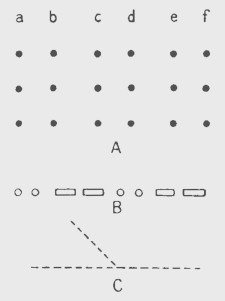
\includegraphics[scale=0.6]{./05_sensible/011}

Fig. 11. Ségrégation des unités
\end{center}
\end{minipage}


— 3° la loi de \textsf{\textit {la bonne forme}} : la forme « prégnante » est toujours « la meilleure»,
c’est-à-dire celle qui présente « le maximum d'unité, de simplicité, de régu-
larité », la mieux structurée, la moins compliquée, la plus symétrique, etc.


\begin{minipage}[c]{.45\linewidth}
\begin{center}
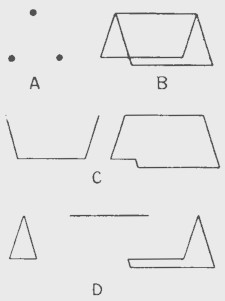
\includegraphics[scale=0.6]{./05_sensible/012}

Fig. 12. La loi de la « bonne forme ».
\end{center}
\end{minipage}
\hfill
\begin{minipage}[c]{.45\linewidth}
Dans la figure 12 A, nous apercevons immédiatement les trois sommets
d’un triangle, et non trois points quelconques ; dans la figure 12 B, deux
parallélogrammes ayant un côté commun, et non un assemblage de figures
compliquées telles que celles des figures 12 C ou 12 D qui pourraient également
la composer.
\end{minipage}


— 4° les lois \textsf{\textit {de la figure et du fond}} : dans un champ
hétérogène, apparaît généralement comme figure : {\it a.} ce qui a un {\it contour}
déterminé, par opposition au fond qui n’en a pas; {\it b.} ce qui est {\it articulé,
différencié,} par opposition au fond qui est plus homogène, plus uniforme ;
{\it c.} ce qui est {\it enveloppé} par le fond : 

\begin{minipage}[c]{.45\linewidth}
\begin{center}
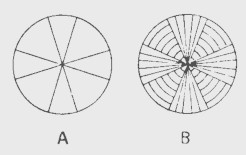
\includegraphics[scale=0.7]{./05_sensible/013}
\end{center}
\end{minipage}
\hfill
\begin{minipage}[c]{.45\linewidth}
\begin{center}
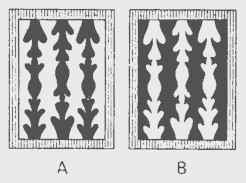
\includegraphics[scale=0.7]{./05_sensible/014}
\end{center}
\end{minipage}
\begin{center}
Fig. 13 et 14. Lois de la figure et du fond.
\end{center}

la figure 13 A est vue comme une croix
%98
à bras minces sur un fond représenté par les secteurs plus ouverts ; {\it d.} ce qui
correspond à certaines {\it directions privilégiées} de l’espace : dans la figure 13 A
l'horizontalité et la verticalité des bras s’ajoutent à l'influence précédente ;
c'est plus net encore dans la figure 13 B où les secteurs sont égaux (remarquer
qu’on a même l'impression, en ce cas, que le fond de cercles concentriques
se continue sous la croix) ;
 {\it e.} ce qui a une structure symétrique par
opposition au fond, qui est asymétrique : dans la figure 14 A, ce sont les
parties noires qui se détachent sur fond blanc parce que leurs contours
%99
sont symétriques par rapport à un axe vertical tandis que, dans la figure 14 B
ce sont les parties blanches qui se détachent sur fond noir pour la même
raison ;

— 5° la loi de transposition : la « forme » peut toujours être « transposée »,
telle une mélodie (exemple cité par Ehrenfels) que l’on reconnaît
facilement malgré une transposition qui change toutes les notes. La transposition
démontre que le tout, comme il a été dit ci-dessus, est indépendant
par rapport aux éléments.
\begin{center}
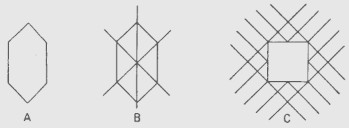
\includegraphics[scale=1.3]{./05_sensible/015}

Fig. 15. — Permanence et camouflage des « formes ».
\end{center}
 D'une façon générale, la « forme » demeure tant
qu’on y introduit des modifications qui n’altèrent pas sa structure primitive
(fig. 15 A et B). Si au contraire on ajoute à une figure des lignes qui
en changent complètement la structure (fig. 15 C), celle-ci n'est plus perçue
dans l’ensemble du dessin, bien qu'elle y soit toujours, parce que d'autres
structures en ont pris la place (carré sur fond quadrillé).}
\vspace{0.31cm}

\section{Discussion du Gestaltisme}% 82.
C'est surtout par réaction
contre l’atomisme psychologique (\S 37) que la Psychologie de la forme,
en tant que {\it psychologie des ensembles}, a connu un très grand succès.
Il y a peut-être cependant un faux dilemme dans l’opposition : ou
bien atomisme des sensations isolées, ou bien « totalités ». Ainsi que
le remarque J. Piaget, « il y a en réalité trois termes possibles : ou
bien une perception est une synthèse d'éléments, ou bien elle constitue
une totalité d’un seul tenant, {\it ou bien elle est un système de rapports} ».
Chaque rapport devient alors lui-même, si l’on veut, une
totalité, mais la totalité d'ensemble devient analysable sans qu'on
soit, pour autant, obligé d’en revenir à l’atomisme, « Cela dit, rien
n'empêche de concevoir les structures totales comme le produit d’une
{\it construction} progressive, procédant, par différenciations accommodatrices
et assimilations combinées, ni de mettre cette construction
en rapport avec une intelligence douée d'activité réelle par opposition
au jeu des structures préétablies » (Piaget).

{\it A.} Un des inconvénients majeurs du Gestaltisme est en effet qu’il
réduit excessivement le rôle de l'{\it activité de l'esprit}. Il prétend tout
ramener à des lois \textbf{\textit {physiologiques}}, réduites elles-mêmes à des lois
%100
d'équilibre \textbf{\textit {physique.}} Köhler admet par exemple que la « forme »
est donnée toute faite dans les perceptions élémentaires grâce à certaines
dispositions anatomiques des nerfs sensitifs (existence de fibres
transversales, etc.). Il y aurait ainsi un {\it principe d’isomorphisme},
d’après lequel, à tout ensemble psychique tel que la perception, correspond
un ensemble physiologique (circuit global de l’objet au cerveau
par les sens). Or il n’y a là qu'hypothèses et « physiologie fantaisiste »
(Janet) imaginée pour les besoins de la cause (tout comme
l'avait fait jadis l’associationnisme). Le « principe d’isomorphisme »
ne fait que restaurer sous sa forme la plus discutable le vieux parallélisme
psycho-physiologique (\S 31 C). Le tout se fonde sur « une
conception vraiment trop simpliste des mécanismes cérébraux » (Piéron) :
si certains phénomènes physiologiques sont ramenés aujourd’hui
à des modèles physiques, il s’en faut qu’ils le soient tous. En
réalité, les faits allégués ne peuvent s'interpréter que du point de
vue d’une biologie beaucoup plus large, où joue notamment la \textbf{\textit {loi
d'économie}} dans l’enregistrement de l'expérience, laquelle explique
« le rôle de la simplicité, de la symétrie, de la régularité » (Piéron)
beaucoup mieux qu’une notion aussi vague et élastique que celle de
la « bonne forme ».

{\it B.} En niant le rôle actif de l’esprit, le Gestaltisme retombe, comme
le remarque encore J. Piaget, dans l’erreur de l’\textbf{\textit {empirisme}} classique
(voir chap. XVII), qui supposait l’ordre rationnel déjà réalisé dans
la nature, de sorte que l’esprit n’aurait plus qu’à l’enregistrer. De la
même façon, le Gestaltisme admet des structures toutes {\it données}, non
seulement dans la réalité physiologique, mais même dans la réalité
physique
{\scriptsize (Certains gestaltistes, comme A. Gelb et K. Goldstein, ont renoncé à cette notion
de « formes » physiques)},
si bien que la perception ne serait plus que « le décalque
d’une réalité externe » (Pradines). On verra bientôt qu’elle est tout
autre chose, à savoir une « structuration des formes » qui suppose «une
activité perceptive dirigée par l'intelligence » (Piaget).

\vspace{0.24cm}
{\footnotesize 
Les cas pathologiques nous montrent d’ailleurs que perception de la
{\it forme} et perception de l’{\it objet} sont relativement indépendantes. « En certains
cas, on constate que la forme est correctement perçue et décrite, alors que
l’objet n’est pas reconnu. D’autres fois, au contraire, avec une perception
des formes très défectueuse, l’objet usuel est indiqué, habilement deviné
et correctement manié » (Piéron). Le premier cas se produit dans les {\it asymbolies}
visuelles ou auditives (cécités ou surdités psychiques), dans lesquelles le
sujet voit ou entend, en apparence, correctement, perçoit des qualités
sensibles, les organise en représentations de forme, de distance, etc., mais
ne reconnaît plus les {\it objets} correspondants, ne sait plus les nommer ni
%101
indiquer par un geste approprié qu'il en connaît le sens et l’usage
{\scriptsize (Tel est le cas célèbre décrit par Gelb et Goldstein en 1918 : un ouvrier de 24 ans,
blessé par éclat d'obus dans la région occipitale, ne {\it reconnaît} plus ce qu'il voit et
cependant est encore capable de différencier les couleurs et les formes (telles que : cercle,
ovale, rectangle, losange). Ces malades sont parfois capables de reconnaître les objets
{\it en raisonnant}. Par exemple, ils arrivent à reconnaître un carré ou un cube au fait
qu'ils présentent des « pointes » ou des angles droits)}.
Le second
cas, celui des {\it astéréognosies}, nous montre des malades incapables de percevoir
les formes et reconnaissant cependant les objets. Il semble même parfois
que, comme le dit Janet, la {\it construction} de la forme soit « une opération
particulière et difficile », car elle disparaît chez des malades affaiblis qui,
encore capables d'accomplir un acte matériellement (manger avec une
cuiller, enfoncer un clou avec un marteau), ne savent plus le mimer avec
l'instrument en main, c’est-à-dire sont devenus « incapables d’exécuter le
même acte quand ils ne doivent en reproduire que la forme ».}
\vspace{0.31cm}

{\it C.} Le Gestaltisme efface toute distinction entre le {\it sensible} et l’{\it intelligible}.
Il « ne fait pas de l’intelligence un domaine séparé ; il rejette
toute distinction de fonctions sensitives et de fonctions intellectuelles »
(P. Guillaume). Or nous avons déjà noté, à propos de
l'enfant (\S 70-71), que voir, entendre, etc., n’est pas nécessairement
{\it comprendre}, et on vient de voir que les cas pathologiques le confirment.
On veut confondre l’intelligible et le sensible ? « Autant dire, répond
Janet, que je dois comprendre immédiatement un texte chinois
puisque le sens est contenu dans les dessins que je vois sur le papier.
Oui, ce sens y est contenu, mais pour un autre qui saura le dégager
en {\it ajoutant} à la perception une opération que je ne peux pas faire. »
Nous retrouvons ici la notion des {\it plans de conscience} (chap. III), que
le Gestaltisme semble bien méconnaître.

D. Cette théorie enfin, sans nier totalement le rôle de l’{\it expérience
antérieure} et de {\it la mémoire}, le sous-estime exagérément, et avec lui
« la réalité du développement {\it génétique} ». Il y a certes, dit Piaget,
« des structures d’ensemble ou {\it formes} dans l'intelligence sensori-motrice
du bébé ; mais loin de demeurer statiques et sans histoire,
elles constituent des {\it schèmes} qui doivent ainsi être accommodées
sans cesse aux situations. Les schèmes ont donc une histoire : il y a
mutuelle réaction entre l’expérience antérieure et l’acte présent d’intelligence ».
Nous croyons, pour notre part, que le rôle propre de
l'intelligence est précisément {\it de donner ainsi une signification} aux
ensembles que nous présentent les sens, en les interprétant, en les
structurant, {\it et cela} en partie {\it d’après notre expérience antérieure}.

\vspace{0.24cm}
{\footnotesize 
Si, dans la figure 12 B, certaines personnes voient un livre posé, à demi
ouvert, sur sa tranche, tandis que d’autres y voient une tente, n’est-ce pas
parce que les premières sont plus familières avec la lecture et les secondes
%102
avec le camping ? Une expérience d'A. Burloud paraît ici décisive : un
dessin formé de rangées parallèles de points en lignes obliques est interprété
par la plupart d’entre nous comme orienté de haut en bas ou de bas en
haut selon la direction des obliques ; mais il est interprété de façon juste
opposée par des étudiants arabes, qui ont l'habitude de lire et d'écrire de
droite à gauche. Nous avons nous-même présenté à une trentaine de personnes
le dessin de la figure 16, qui est un dessin de tapisserie, en leur
demandant de dire ce qu’elles y voyaient immédiatement et sans réflexion.

\begin{center}
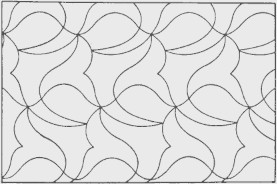
\includegraphics[scale=1.3]{./05_sensible/016}

Fig. 16. — La perception des « formes ».

{\it Que voyez-vous dans ce dessin de tapisserie ?}
\end{center}

Il est remarquable qu'aucune d’entre elles n’a indiqué l’espèce de sinusoïde
qui est cependant la « forme » la plus simple du dessin. Presque toutes y
ont vu « des fleurs » mêlées à des dessins de fantaisie. Un enfant de cinq ans
y a aperçu « des queues de poisson ». Un adulte y a discerné « des sortes de
crocs ou d’enclumes de cordonnier ». Il est évident que des {\it schèmes} perceptifs
dus à l'expérience antérieure viennent s’interposer ici entre le donné
sensible et l'interprétation perceptive.}
\vspace{0.31cm}

\section{Du syncrétisme aux objets distincts}% 83.
{\it A.} Ce qu’on peut
retenir de la théorie de la Forme, c’est que la perception ne part pas,
chez l’enfant, d'éléments isolés, mais de certains {\it ensembles} et que ces
ensembles {\it ne sont pas}, primitivement, des ensembles {\it analysés} ni des
ensembles {\it construits} : ils sont perçus \textbf{\textit {syncrétiquement.}}

\vspace{0.24cm}
{\footnotesize 
Quelques exemples feront mieux comprendre en quoi consiste ce syncrétisme.
Claparède cite le cas d’un enfant de 4 ans à qui l’on avait appris
les {\it Rondes enfantines} de Dalcroze, sa mère l’accompagnant au piano.
Quelques semaines après le début de l'apprentissage, l'enfant sait ouvrir
l’album à la page voulue pour demander qu'on lui joue telle ronde déterminée.
%103
Nous avons constaté nous-même qu’un enfant de 4 ans sait parfaitement
distinguer, parmi un assez grand nombre d’autres, un disque de
phonographe à son étiquette. Voici enfin un cas particulièrement typique :
on montre à un enfant de 5 ans quarante et une images représentant les
facteurs de pays différents, avec, dans les coins, un timbre-poste et le
drapeau du pays correspondant ; l’enfant apprend très vite les noms des
41 pays. Après une interruption de trois mois, il sait les dire encore pour
13 images. On lui demande à quoi il les reconnaît. Il déclare tantôt que
c’est grâce au timbre, tantôt que c’est grâce au drapeau, tantôt enfin au
képi du facteur. Or {\it il reconnaît encore les images quand ces détails sont
cachés}. En réalité, un syncrétisme s’est établi entre les noms de pays qu’on
lui a appris et «la physionomie générale de l’image »
{\scriptsize (Il est à remarquer que cet exemple de T. Jonckheere, comme celui de Claparède,
est cité dans les {\it Archives de psychologie} de 1908, donc bien avant le développement des
théories gestaltistes)}.}
\vspace{0.31cm}

Ce syncrétisme n’est pas, à proprement parler, une perception
structurée, organisée, comme le voudrait le Gestaltisme. L’enfant ne
prend pas conscience des rapports. Il est, commentait Claparède,
« dans le même état d’esprit qu’un adulte qui ignore et qui ne sait pas
qu’il ignore. Il n'analyse pas ce qu’il a sous les yeux, si les parties
du tout qu'il observe lui sont encore inconnues ou ne suscitent pas
son intérêt d'une façon particulière ». C’est à peu près dans le même
sens que H. Piéron a dit que, dans un jardin ensoleillé où dort un
chien, ce que le tout jeune enfant perçoit d’abord, c’est l’ensemble :
{\it le jardin-au-soleil-avec-le-chien}. « De cet ensemble, le jardin, le
chien et le soleil se dissocieront comme réalités indépendantes,
puis l’aboiement, la toison du chien s’individualiseront. » Comment
va s’opérer cette dissociation ? Comment vont se dégager les objets
perçus ?

{\it B.} Remarquons d'abord que la loi du syncrétisme ne vaut pas
{\it également} pour tous les sens. Ainsi que le note J. DeLay, les Gestaltistes
« n'ont guère étudié les lois du complexe de la Forme que dans
le domaine optique. Or il y a une différence fondamentale entre les
“ formes ” optiques et les “ formes ” tactiles. Dans le domaine visuel,
la perception du tout est aussi immédiate que la perception des
parties et même elle la précède. Dans le domaine \textbf{\textit {tactile,}} le complexe
ne naît que par synthèse active des formes élémentaires et partielles ».

{\it C.} Chez l’homme, le toucher présente d’ailleurs une importance
toute particulière du fait qu’il est l’organe principal de l’\textbf{\textit {action}} sur
le monde extérieur, et l’on ne saurait trop insister à ce propos sur le rôle
de la {\it main} dans la représentation que nous nous faisons des objets :
les animaux qui ne disposent pas d’une main préhensive ne perçoivent
%104
pas les choses comme nous. Mais il y a lieu de généraliser :
« {\it Reconnaître un objet usuel}, a dit Bergson, {\it consiste surtout à savoir
s’en servir}. » La perception a d’abord une fonction pratique : son
rôle est de « préparer des actions » ; elle est « la mesure de notre
action possible sur les corps » ; et elle ne retient du réel que ce qui est
utile à notre action présente. « Le monde est peut-être, dit encore
Bergson, une continuité indistincte. Chaque êtke découpe le monde
selon les lignes mêmes que son action doit suivre. » On a vu (\S 40)
que l’enfant définit d’abord les objets par l’{\it usage}. Mais nous-mêmes
que percevons-nous d’abord dans un crayon ou un stylo, sinon l’objet
qui sert à écrire ? dans un couteau, sinon l’objet qui sert à couper ?
dans une chaise ou un fauteuil, sinon l’objet qui sert à s’asseoir ?
N'est-ce pas ce rapport avec notre {\it action} qui fait pour nous l’unité de
l’objet, beaucoup plus que sa « forme » au sens gestaltiste ?

{\it D.} Plus généralement encore, il faut invoquer ici \textbf{\textit {l’intérêt affectif,}}
lui-même en relation avec nos {\it besoins} et nos {\it tendances}. « L'unité de
l’objet est déterminée par un acte particulier qui dépend des besoins
et des tendances de l’organisme. C’est le besoin de boire qui donne
naissance à l’objet que nous appelons de l’eau. C’est le besoin de
manger et la tendance à manger qui donne de l’unité au fruit. Ce qui
établit l’unité et la physionomie d’une chose, c’est la satisfaction ou
l’insatisfaction directe ou indirecte de nos tendances » (Janet). Chez
le nouveau-né, c’est l'intérêt qui, du syncrétisme primitif, fait surgir
quelques ensembles individualisés : la maman ou la nourrice, le
biberon, etc. Autrement dit, il y a, selon l’expression de Piaget,
« assimilation des choses aux {\it schèmes} (héréditaires ou acquis) du sujet » :
ces schèmes sont par exemple ceux de la succion, de la vision, de la
préhension. Mais, à ce stade, l’univers consiste beaucoup moins en
objets permanents qu’« en tableaux perceptifs mobiles et plastiques,
centrés sur l’activité propre » (voir \S 102).

\vspace{0.24cm}
{\footnotesize 
Cette structure mentale égocentrique du tout jeune enfant se traduit
encore plus tard dans ses {\it dessins}. G. Luquet avait déjà montré que, chez
l’enfant, « l'intention de dessiner tel objet n’est que le prolongement et la
manifestation de sa représentation mentale ». L'enfant dessine, non ce qu’il
a sous les yeux, mais un {\it type} : le bonhomme, la maison, etc., qui « correspond
à une réalité psychique existant dans son esprit », et qui constitue un
véritable {\it modèle mental}. Autrement dit, il dessine {\it ce qu’il sait}, non ce qu'il
voit : ainsi, dans une sonnette à main posée sur une table, il dessine le
battant, quoique celui-ci ne soit pas visible, parce qu'il {\it sait} qu'il existe
(fig. 17). Une étude plus récente de M. Prudhommeau (sur {\it Le dessin de
l'enfant}) a confirmé ce résultat ; mais elle a montré en même temps combien
est complexe le passage de ce réalisme intellectuel au réalisme visuel.
Les premiers dessins de l'enfant relèvent uniquement du réalisme intellectuel : 
our figurer « un bonhomme », il commence par dessiner le classique
%105
« bonhomme tétard » qui est « {\it la projection de l’image qu'il se fait de son
corps} », {\it des postures qu’il parvient à dominer lui-même} dans son équilibre
interne et externe. Le réalisme visuel qui apparaît vers 8-9 ans implique au
contraire la prise de conscience {\it objective} des rapports posturaux corrects.

\begin{center}
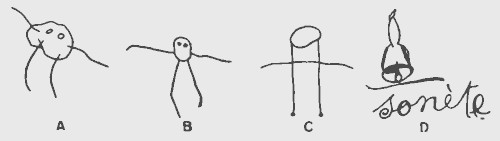
\includegraphics[scale=0.9]{./05_sensible/017}

Fig. 17. — Le dessin enfantin.

(D’après Luquet, {\it Les dessins d'un enfant},

et Prudhommeau, {\it Le dessin de l'enfant}, P. U. F., éd.).
\end{center}

A et B. {\it Bonshommes tétards dessinés par des enfants de 3 ans 1/2 : l'enfant dessine d’abord
une tête à laquelle sont directement attachés les bras (quand il les dessine) et les jambes.
Mais cetle tête symbolise, en réalité, pour lui « l'ensemble du corps humain »} (Prudhommeau).
— {\it C'est ce que montre bien le dessin C (enfant de 4 ans, 1 mois) où les bras sont
attachés aux jambes, avec un trait horizontal qui est peut-être déjà une ébauche de figuration
du tronc. Ce n'est que vers 5 ans que celui-ci apparaît de façon distincte}. — D. {\it Dessin
d'une sonnette par un enfant de 7 ans 4 mois}.}
\vspace{0.31cm}

\section{La construction des objets}% 84.
Il importe d'ajouter que,
dans la constitution des objets, il intervient ainsi un processus de
{\it construction} (et non seulement de dissociation), fonction de l’expérience
acquise, ce que la théorie gestaltiste risquerait de nous faire
méconnaître. Un objet est un complexus de propriétés qui, le plus
souvent, intéressent {\it différents sens}. Or il n’y a pas {\it a priori} de liaison
nécessaire — quoique, pour l’enfant, il y ait souvent un lien syncrétique,
mais arbitraire
{\scriptsize (Un enfant dira volontiers que « les gâteaux roses » ou « les bonbons rouges », c'est
bon. — Nous avons fait l'observation suivante sur un enfant d'environ cinq mois.
Alors qu’il commence à faire jour, un réveille-matin, tout à côté duquel se trouve une
veilleuse encore allumée, se met à sonner. L'enfant, déjà éveillé, regarde avec un étonnement
évident, non le réveil, mais la veilleuse, quoique de son berceau il puisse voir
les deux)}
 — entre ces différentes qualités sensibles :
entre la couleur et la saveur par exemple. Nous avons, de l’univers
qui nous entoure, un « atlas tactile » et un « atlas visuel », comme
disait Taine, et les observations faites sur les aveugles-nés opérés et
devenus voyants montrent qu’ils se trouvent parfois tout à fait
dépaysés dans ce monde visuel nouveau pour eux et qui n’a pas, en
principe, de commune mesure avec le monde tactile auquel ils sont
habitués : on a souvent cité l’exemple du jeune aveugle opéré par le
%106
chirurgien anglais Cheselden (1728) qui ne pouvait distinguer le chat
et le chien de la maison, qu’il connaissait bien par le toucher, jusqu’au
jour où il les caressa et regarda en même temps. La jonction de ces
différents « atlas » se fait peu à peu par l’expérience et souvent l'{\it expérience
active} (chez l’enfant, à partir de l’âge de 4-5 mois, palpation,
manipulation des objets, en même temps qu'il les regarde, les écoute
s’ils font du bruit, etc.). On verra plus loin que cette {\it construction} peut
se poursuivre jusque chez l’adulte sous la forme de ce qu’on appelle
les « perceptions acquises » (\S 87 B).

\section{Les cadres sociaux de la perception}% 85.
L'homme, rappelons-le
(\S 24 et 32), est un {\it être social}, et le monde qu’il se construit,
est fonction non seulement de l’être vital, mais aussi de l être social
qui est en lui. L. Lévy-Bruhl a pu écrire que « les primitifs ne perçoivent
rien comme nous », non que leurs sens ou leur appareil cérébral
soient différents des nôtres, mais parce que des \textbf{\textit {représentations
collectives}} différentes des nôtres viennent se mêler chez eux à la
perception ou plutôt en sont « partie intégrante ». Quel que soit
l'objet qui se présente à eux, il implique des propriétés « mystiques »,
comme dit Lévy-Bruhl, disons plutôt : magiques. Pour eux, « il
n’y a pas de fait proprement physique, au sens que nous donnons à
ce mot » : tout ce qu’ils perçoivent, l'eau qui coule, le vent qui souffle,
la pluie qui tombe, un son, une couleur, implique des « participations »
mystérieuses, des propriétés invisibles. Comme le remarquait
Ch. Blondel, « entre les primitifs et nous, l'humanité a passé par
toute une série de visions collectives du monde où la conception de
la réalité s’est graduellement dépouillée de ce caractère mystique
pour se faire de plus en plus positive ». — En fait, ainsi que le remarquait
récemment L. Goldmann (à propos de la peinture de Chagall)
« tout groupe social, orienté vers une organisation globale de la société,
tend à élaborer une vision cohérente [c’est-à-dire universelle] du
monde qui, étant donné que les innombrables distorsions individuelles
s’annulent les unes les autres, est mieux réalisée et, par cela, plus facile
à saisir dans le groupe que chez la plupart de ses membres pris individuellement. »

Blondel observait encore que le monde dans lequel vit l’homme
moderne n’est pas fait d'objets naturels, mais d'\textbf{\textit {objets fabriqués,}}
produits d’une certaine technique. Or « l'interprétation de la plupart
d’entre ces objets implique une initiation sociale. Quand nous
disons : voici un chapelet ou voici un appareil téléphonique, notre
affirmation dépasse énormément la simple constatation des formes
en effet perçues, elle suppose une connaissance de techniques religieuses
%107
ou scientifiques que nous devons uniquement à notre milieu ».

À plus forte raison en est-il ainsi des \textbf{\textit {symboles}} ou des \textbf{\textit {emblèmes.}}
« Au premier coup d'œil, nous percevons quelle profession ou quel
commerce s’exercent dans les boutiques ou les maisons des rues que
nous parcourons, à des particularités d’ornementation ou de disposition
qui, variables en général d’un pays à l’autre, sont toutes
conventionnelles et symboliques, tels en France l’écusson des notaires,
la carotte des bureaux de tabac ou [jadis] le plat à barbe des coiffeurs »
(Blondel). Qu'on songe au nombre de conventions qu’implique un
simple {\it signal}, comme les signaux qui règlent la circulation dans les
rues d’une ville et, bien plus encore, à l’ensemble de {\it croyances}, de {\it sentiments},
de {\it traditions} que représente un emblème, tel que le drapeau,
la croix ou le croissant !

Ajoutons que la perception de l’objet est liée pour nous à son
\textbf{\textit {nom,}} à tel point qu’on pourrait dire : « {\it Reconnaître un objet consiste à
savoir le nommer}. » L'enfant, comme le remarque E. Cassirer, a
une véritable « faim de noms », mais ce n’est pas que son intérêt
s'attache « à l’acte de désignation, que d’ailleurs il ignore encore
complètement en tant qu’acte isolé ». Il demande le nom « pour prendre
en quelque sorte par lui possession de la conscience de la chose: il se
produit entre la chose et le nom une véritable {\it concrescence} ». Pour lui
comme pour le primitif, « le mot est un élément objectif de la chose
et constitue son essence propre ». Même chez nous, le nom donné à
l’objet réagit sur la représentation que nous nous en faisons. Plus
généralement, le nom de l’objet « l’attire avec lui dans ce monde de
relâtions logiques qu’est précisément le monde de nos mots » ; car,
étant généralement un nom commun, il « affirme à la fois qu’outre
ses céractères individuels l’objet nommé en possède d’autres qui
l’apparentent aux objets de la même espèce et que, faisant partie
d’une espèce, il se situe à une place définie dans l’ensemble de notre
expérience et des notions où elle trouve son unité » (Blondel).
Autrement dit, nommer un objet, c’est le {\it classer}, c’est-à-dire l'intégrer
à toute une représentation du monde cristallisée dans le {\it langage}.

Il faut tenir compte enfin des dispositions mentales créées par la
\textbf{\textit {situation sociale}} du sujet. « L'agent de police, l’assistante sociale, le
politicien de clocher, le touriste étranger qui se promènent dans le
même quartier de taudis, non seulement interprètent différemment
ce qu’ils voient, mais encore perçoivent vraiment des choses différentes »
(Krech et Crutchfield).

\section{La perception individualisée}% 86.
Les facteurs de dissociation
et de construction examinés jusqu'ici ne nous donnent encore
%108
qu’une perception {\it générique} des objets : l’usage pratique ou social
caractérise toute une {\it classe} d'objets, et le nom, remarquions-nous,
est {\it commun}. Comment parviendrons-nous de là à la perception \textbf{\textit {individualisée,
singulière ?}}

« Il y a perception singulière des êtres concrets, personnes ou choses,
lorsque notre perception nous apporte la connaissance non de l'espèce
à laquelle son objet appartient, mais celle de cet objet lui-même, discerné
comme tel de tous les objets du même genre » (Blondel). Or
certains malades (syndrome dit de Korsakoff) sont capables d’identifier
les données de leurs perceptions, mais non plus de les individualiser :
« Ils savent qu’ils sont dans un hôpital, mais, d’un jour à
l’autre, d’un instant à l’autre, ils sont hors d’état de reconnaître
qu’ils sont dans le même hôpital. Ils savent qu’ils parlent à un
médecin, mais, si répétées qu’aient été leurs rencontres avec lui, il
demeure toujours pour eux un nouveau venu. » L'étude des dessins
d’enfants montre que c’est seulement à partir d’un certain âge qu’apparaissent
« les dessins figurant des motifs individuels nettement spécialisés
par leurs détails distinctifs » ; que l’enfant dessine par exemple
non plus {\it la} maison en général, mais {\it une} maison qu'il a devant lui.
Tout ceci prouve que la perception personnelle et, comme dit Blondel,
« historique » — car elle implique la conscience de notre « histoire »,
du passé propre à chacun de nous — est une opération relativement
indépendante et qui met en jeu des fonctions élevées. Ce qui vient
d’être dit montre qu’elle suppose la \textbf{\textit {mémoire}} : il suffit parfois que
nous revoyions un livre, un paysage, une photo pour que toute une
scène de notre vie passée revienne à notre esprit. Elle suppose aussi
l'\textbf{\textit {attention}} : la reconnaissance d’un objet n’est possible qu’à l’aide
de ces {\it préperceptions} dont il a été question au \S 49 D. Elle suppose
enfin le \textbf{\textit {jugement.}} À vrai dire, pour les objets familiers, ce jugement
demeure le plus souvent implicite : il est à rapprocher de ces « jugements
naturels » qui, selon Malebranche, se font « en nous sans nous
et même malgré nous » et qui produisent des « sensations composées ».
Dans certains cas cependant, lorsque nous hésitons à identifier ce
que nous voyons de loin, ce que nous entendons sourdement, ce que
nous touchons dans une pièce obscure où nous nous déplaçons à
tâtons, nous prenons mieux conscience de l’{\it assertion} impliquée dans
la perception. Ainsi, nous voyons un point blanc sur la mer : nous
{\it jugeons} que c’est un bateau à voile ; nous entendons un crépitement
sur la vitre : nous {\it jugeons} qu’il pleut, ete. — La perception nous
apparaît ainsi comme étant déjà un véritable \textbf{\textit {acte intellectuel}}
({\it Exercice} 7).

%109
\section{« L'éducation des sens »}% 87.
Si la perception est, en partie,
construite, il en résulte que notre faculté de perception peut être,
dans une certaine mesure, éduquée. Il est cependant nécessaire de
distinguer ici comme deux plans différents.

{\it A.} Sur le plan de la \textbf{\textit {sensation}} proprement dite, une certaine éducation
est déjà possible par laquelle nos sens peuvent être {\it affinés},
acquérir une {\it acuité} (\S 78) supérieure. On dit que l’ouvrier des Gobelins
parvient à discerner plus de deux mille nuances différentes de vert :
ceci est évidemment acquis, non inné. Il y a lieu d’insister de nouveau
ici sur le rôle de l’{\it attention} dans une telle éducation : bien des gens se
plaignent d’avoir une mauvaise mémoire des couleurs, qui n’ont
jamais regardé attentivement la nature
{\scriptsize (C'est peut-être là ce qui fait la différence entre la perception chez l’homme et la
perception chez la femme. G. Heymans dit, dans sa {\it Psychologie des femmes}, que la
femme donne l'impression de percevoir plus finement que l’homme, alors qu’à l'examen
c'est plutôt le contraire qui apparaît comme vrai. La solution, ajoute-t-il, est dans cette
réflexion de Mme de Rémusat : « Apercevoir nous va mieux qu’observer. » La perception
spontanée est effectivement plus fine, mais c'est l'attention qui manque)}.
L’attention sensorielle
(\S 48) fait au contraire apercevoir dans un objet quantité de détails
ou d’aspects que nous n’y aurions jamais remarqués sans elle. C’est
grâce à elle que l’artiste se libère des perceptions clichées, stéréo-typées,
tout utilitaires, du sens commun pour {\it individualiser} sa vision
du monde et retrouver ainsi la sensation première dans toute son
originalité et sa fraîcheur (voir {\it Exercice} 6).

B. Mais l’éducation dite « des sens » est surtout, au vrai, une éducation
{\it de la perception}, qui consiste à enrichir la {\it signification} des
données d’un sens {\it de qualités relevant d’autres sens} ou même d’enseignements
plus généraux : ce sont les \textbf{\textit {perceptions acquises.}}

\vspace{0.24cm}
{\footnotesize 
Nous apprenons à juger à la couleur ou à l’odeur d’un fruit s’il est mûr ou
non, au toucher d’une étoffe si elle est en laine ou en coton, au son d’un
récipient s’il est vide ou plein, etc. « Tel distinguera à leur saveur la moitié
supérieure et la moitié inférieure d’une bouteille de vieux madère. Tel autre,
rien qu’à plonger sa main dans de la farine, vous dira si elle vient du Iowa
ou de Tennessee. Laura Bridgman, la sourde-muette-aveugle, avait le toucher
assez fin pour reconnaître à un an d'intervalle la main d’une personne
qui lui avait donné une poignée de main » (James). Un personnage de
Giraudoux reconnait, la nuit, au pas d’un paysan, de quel village il est, et
Marcel Proust, en s’éveillant, sait, aux bruits de la rue, quel temps il fait
({\it Exercice} 9). C'est ainsi encore qu’à la couleur d’un précipité le chimiste
détermine la nature d’un corps ; le médecin se sert de la palpation et de
l’auscultation pour apprécier l'état des organes ; au timbre de voix d’un
interlocuteur, nous discernons s’il est ému ou calme; etc.}
\vspace{0.31cm}

À vrai dire, « l’éducation des sens » se confond ici avec le développement
intellectuel : « Savoir regarder, dit P.-M. Schuhl, c’est tout
%110
le secret de l’invention scientifique, du diagnostic-éclair des grands
cliniciens, du “ coup d'œil ” des vrais stratèges. »

\section{Les erreurs de la perception}% 88.
La perception, étant une
opération complexe et, en partie, intellectuelle, est susceptible d’erreurs.
C’est ce qu’on a appelé les {\it erreurs des sens}, mais l’expression
est impropre : « Ce ne sont pas nos sens qui nous trompent, dit
Malebranche, mais c'est notre volonté qui nous trompe par ses
jugements précipités. » Il se glisse toujours en effet dans ces erreurs un
minimum d'\textbf{\textit {interprétation,}} donc, comme le dit Malebranche, de
\textbf{\textit {jugement,}} ne serait-ce que ce jugement erroné (\S 79) que nos sensations
sont les copies ou les images des réalités extérieures. — On peut
distinguer deux cas : tantôt l’erreur porte sur {\it un des caractères} de
l’objet, tantôt elle porte sur son {\it identité} même.

{\it A.} Dans le premier cas, l’erreur peut porter : sur la {\it forme} spatiale
de l’objet (cas du bâton à demi plongé dans l’eau et que l’on « voit »
brisé), sur sa {\it couleur} (phénomènes de contraste signalés au \S 73 C),
sur le {\it nombre} des objets perçus (expérience dite d’Aristote : si l’on
fait rouler une bille entre l'index et le médius préalablement croisés,
on sent deux billes au lieu d’une), sur leur {\it poids} relatif (illusion de
Demoor : de deux poids égaux, celui qui a le plus petit volume paraît
le plus lourd, même si les deux poids sont soupesés à l’aide d’anneaux
identiques), etc. Dans tous ces cas, il n’est pas difficile de découvrir
{\it un jugement implicite} : nous jugeons de la forme du bâton {\it comme
s’il était plongé dans un seul milieu réfringent}, l'air, ainsi qu’il arrive
en effet le plus souvent pour les objets que nous percevons ; dans
l'expérience d’Aristote, nous jugeons {\it comme si nos doigts étaient
dans leur position normale} ; l'illusion de Demoor n’existe ni chez le
tout jeune enfant ni chez le dégénéré : seul l’adulte normal se trompe
parce que, chez lui, l’appréciation ordinaire du rapport volume-poids
a fini par s’incorporer à la perception elle-même. — La plupart des
illusions d’optique s’expliquent ainsi par des phénomènes accessoires
provoquant des interprétations spontanées : un trompe-l’œil est toujours
un «trompe-l’esprit ».

\vspace{0.24cm}
{\footnotesize 
Dans la figure 18 A, c’est un phénomène d'{\it irradiation}, lequel fait que le
carré blanc empiète sur la rétine en dehors de sa propre zone, ce qui le fait
juger plus grand. Dans les figures 18 B et C, c’est l’action des {\it obliques},
qui provoquent des {\it mouvements} de l'œil brisant le parallélisme. Dans
18 D, ce sont les côtés des triangles semblables que l’œil a tendance à
suivre, ce qui déforme la circonférence. Enfin les figures 18 E et F donnent
des exemples des illusions de relief (\S 96).}
\vspace{0.31cm}
\begin{center}
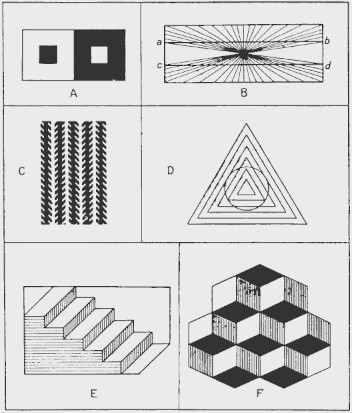
\includegraphics[scale=0.7]{./05_sensible/018}

Fig. 18. — Quelques illusions d'optique.
\end{center}
A. {\it Les petits carrés blanc et noir sont égaux}. — B. {\it Figure de Hering} : a b {\it et} c d {\it sont droites
et parallèles}. — C. {\it Figure de Zollner : les verticales coupées par des obliques sont parallèles}.
— D. {\it Figure de Gatti : cercle déformé par les triangles}. — E {\it et} F. {\it Illusions de
relief} (E, {\it escalier de Schrüder} ; F, {\it on voit tantôt 6, tantôt 7 cubes}).

%111
{\it }B. Dans le second cas, celui des illusions proprement dites, {\it nous prenons
un objet pour un autre, une personne pour une autre}. Ici l’interprétation
surajoutée aux données sensibles est évidente, d’autant
plus qu’elle est généralement en relation avec {\it un état global de la
conscience}. Si de loin nous prenons une personne quelconque pour

%112
un de nos amis, c’est bien souvent parce que nous attendons celui-ci.
Si le peureux voit, la nuit, dans les buissons ou les arbres de la route,
des fantômes ou des brigands, c’est précisément parce qu’il est peureux.
Un passant voit, à ‘la devanture d’un libraire, des livres traitant
de sciences occultes et, à côté, des livres d'histoire parmi lesquels
1815 de Henri Houssaye ; au lieu de 1815, il lit ISIS (les mystères
d’Isis sont connus des occultistes). Regardant par la fenêtre, Edgar
Poë croit voir un animal gigantesque marcher sur la crête d’une colline
qui se profile à l’horizon (au lieu d’un moucheron qui se promène
sur la vitre). Mais son amour du fantastique n’y est-il pour rien?

(Phot. Bibl. Nat.)

\begin{center}
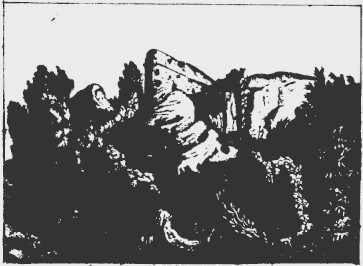
\includegraphics[scale=0.7]{./05_sensible/019}

Fig. 19. — Une estampe amusante.
\end{center}

{\it Au {\footnotesize XVIII}$^\text{e}$ siècle s'était répandue la vogue des « estampes amusantes », notamment de celles
qui présentent un double sens. La gravure ci-dessus prétend représenter le château de
la ville de Pépa, comitat de Veszprem, en Hongrie. Mais, si on la place sur le côté gauche,
dans le sens de la hauteur, elle apparaît tout autrement.}

%113
On trouvera de nombreux exemples de ces illusions dans les œuvres de
Marcel Proust. Tantôt, au bord de la mer, il aperçoit au loin une ligne
blanche qu'il prend pour une chaussée de pierres ou une digue : c’est seulement
lorsqu'il voit un navire s’y aventurer qu'il comprend que c’est une
frange d'écume. Tantôt, le matin au réveil, apercevant une lueur allongée
à un certain endroit de sa chambre, il croit que c’est le jour qui commence à
filtrer sous les rideaux de la fenêtre : c'est une tringle de cuivre devant la
cheminée, où se reflète une dernière braise du foyer. L'idée qu’il doit commencer
à faire jour est ici à la base de l'erreur.

Un phénomène analogue se produit dans les images à sens multiples
ou les images-devinettes, telles que celles des figures 8, 17 {\it E} et {\it F}
et 19 : il est très remarquable qu’à un moment donné c’est {\it une}
interprétation qui s'impose ; le passage à {\it une autre} interprétation
se fait brusquement. Il y a bien ici, sinon tout à fait une « forme »
au sens gestaltiste, du moins un « modèle mental », une orientation
de l'esprit à la base de l'interprétation.

\section{Sujets de travaux}% SUJETS DE TRAVAUX

{\bf Exercices.} — 1. {\it Analyser introspectivement la sensation kinésique en
distinguant} : a. {\it la sensation} musculaire ({\it par exemple, quand on contracte le
biceps en laissant l'avant-bras immobile}) ; b. {\it la sensation} tendineuse ({\it en
crispant la main comme pour griffer quelqu'un}) ; c. {\it la sensation} articulaire
({\it en faisant tourner la main autour du poignet, le coude étant posé sur une
table}). — 2. {\it Observez le phénomène de la} vision crépusculaire. — 3. {\it Expliquez
et commentez ce texte d'A. Gide :} « La vue — le plus désolant de nos sens.
Tout ce que nous ne pouvons pas toucher nous désole ; l'esprit saisit plus
aisément la pensée que notre main ce que notre œil convoite. » — 4. {\it Commenter
cette phrase de Van Gogh :} « Cette combinaison d'ocre rouge, de
vert attristé de gris, de traits noirs qui cernent les couleurs, cela produit
un peu la sensation d'angoisse dont souffrent souvent certains de mes
compagnons d'infortune et qu'on appelle {\it noir-rouge}. » — 5. {\it Comment
comprenez-vous ce mot de Ruskin} : « L’essence de la vulgarité réside dans
l'absence de sensations » ? — 6. {\it Commentez cette citation d’Eugène Delacroix :}
« La loi du vert pour le reflet et du bord d'ombre ou de l'ombre portée, que
j'ai découverte antérieurement dans le linge, s'étend à tout comme les
trois couleurs mixtes [orangé, vert, violet] se retrouvent dans tout... Sur
la mer, c’est aussi évident. Les ombres portées évidemment violettes,
et les reflets toujours verts, aussi évidemment. » — 7. {\it Expliquez ce jugement
d'Alain :} « La perception est déjà une fonction d’entendement..., l'esprit
le plus raisonnable y met de lui-même bien plus qu'il ne croit. » — 8. {\it Commentez
ce texte de Marcel Proust :} « Dès le matin, la tête encore tournée contre
le mur, je savais déjà le temps qu'il faisait. Les premiers bruits de la rue
me l'avaient appris selon qu’ils me parvenaient amortis et déviés par
l'humidité ou. vibrants comme des flèches dans l'aire résonnante et vide
d'un matin spacieux, glacial et pur ; dès le roulement du premier tramway,
j'avais entendu s’il était morfondu dans la pluie ou en partance pour
l'azur. » — 9. {\it Cherchez et analysez quelques exemples d'illusions sensorielles
(auditives notamment) analogues à celles du \S 88 A.}

%114

{\bf Exposés oraux.} — 1. {\it Le caractère purement qualitatif de la sensation et la
critique de la Psychophysique}, d’après Bergson, chap. I. {\it Discussion} (voir
Pradines, p. 417-453). — 2. {\it La théorie de la Forme, appliquée à la perception,}
d’après GuiLLaume.

{\bf Discussions.} — 1. {\it La distinction entre} sensation {\it et} perception {\it a-t-elle
perdu toute valeur ?} — 2. {\it Discuter ce passage de J.-P. Sartre :} « Certains
rouges de Matisse provoquent une jouissance sensuelle chez celui qui
les voit. Mais cette jouissance, si on la considère isolément — par exemple,
si elle est provoquée par un rouge donné en fait dans la nature — n’a rien
d'esthétique. C’est purement et simplement un plaisir des sens. Lorsqu'on
saisit, au contraire, le rouge sur le tableau, on le saisit malgré tout comme
faisant partie d’un ensemble irréel et c’est dans cet ensemble qu’il est beau. »

{\bf Lectures.} — {\it a.} Bergson, {\it Les Données immédiates de la conscience}, Alcan,
1888, chap. I. — {\it b.} Ch. Blondel, {\it Introd. à la psychologie collective}, coll.
A. Colin, 1928, 2$^\text{e}$ partie, chap. I. — {\it c.} M. Pradines, {\it Philosophie de la
sensation}, Belles-Lettres, 1928 ; et {\it d. Traité de Psychologie générale},
P. U. F., 1943, tome I, p. 399-470 et 497-538. — {\it e.} G. Dumas, {\it Nouveau
Traité de Psychologie}, Alcan, 1932-1936, tome II, liv. II, et tome V, p. 1-75
et 79-84 (B. Bourdon). — {\it f.} E. Cassirer, {\it Le langage et la construction du
monde des objets}, dans le {\it Journal de Psychologie}, année 1933, p. 18. —
{\it g.} P. Janet, {\it Les Débuts de l'intelligence}, Flammarion, 1935, 2$^\text{e}$ partie,
chap. V. — {\it h.} P. Guillaume, {\it La Psychologie de la forme}, Flammarion,
1937, chap. III. — {\it i.} P. Chauchard, {\it Les Messages de nos sens}, P. U. F.,
1944. — {\it j.} M. Merleau-Ponty, {\it Phénoménologie de la perception}, Gallimard,
1945. — {\it k.} H. Piéron, {\it La Sensation, guide de vie}, Gallimard, 1945.
— {\it l.} J. Piaget, {\it Psychologie de l'intelligence}, coll. A. Colin, 1947, chap. III. —
{\it m.} D. Krech et R. S. Crutchfield, {\it Théorie et problèmes de Psychologie
sociale}, P. U. F., 1952, chap. III et IV. — {\it n.} J. Piaget, {\it Les mécanismes
perceptifs}, P. U. F., 1961. — {\it o.} Paul Fraisse et J. Piaget, {\it Traité de Psychologie
expérimentale}, fasc. II : {\it Sensation et motricité}, par Pieron, Chocolle
et Leplat, et fasc. VI : {\it La Perception}, par Piaget, Fraisse, Vurpillot
et Francès, P. U. F., 1963. — {\it p.} Robert Francès, {\it La Perception}, P. U. F.,
1964. — {\it q.} H. Gratiot-Alphandéry et R. Zazzo, {\it Traité de psychologie de
l'enfant}, 3 vol., P. U. F., 1970.
